\documentclass[12pt]{article}
\usepackage{lmodern}
\usepackage{amsmath}
\usepackage{ifxetex,ifluatex}
\ifnum 0\ifxetex 1\fi\ifluatex 1\fi=0 % if pdftex
  \usepackage[T1]{fontenc}
  \usepackage[utf8]{inputenc}
  \usepackage{textcomp} % provide euro and other symbols
  \usepackage{amssymb}
\else % if luatex or xetex
  \usepackage{unicode-math}
  \defaultfontfeatures{Scale=MatchLowercase}
  \defaultfontfeatures[\rmfamily]{Ligatures=TeX,Scale=1}
\fi
% Use upquote if available, for straight quotes in verbatim environments
\IfFileExists{upquote.sty}{\usepackage{upquote}}{}
\IfFileExists{microtype.sty}{% use microtype if available
  \usepackage[]{microtype}
  \UseMicrotypeSet[protrusion]{basicmath} % disable protrusion for tt fonts
}{}
\makeatletter
\@ifundefined{KOMAClassName}{% if non-KOMA class
  \IfFileExists{parskip.sty}{%
    \usepackage{parskip}
  }{% else
    \setlength{\parindent}{0pt}
    \setlength{\parskip}{6pt plus 2pt minus 1pt}}
}{% if KOMA class
  \KOMAoptions{parskip=half}}
\makeatother
\usepackage{xcolor}
\IfFileExists{xurl.sty}{\usepackage{xurl}}{} % add URL line breaks if available
\IfFileExists{bookmark.sty}{\usepackage{bookmark}}{\usepackage{hyperref}}
\hypersetup{
  pdftitle={Memories of migrations past: Sociality and cognition in dynamic, seasonal environments},
  pdfauthor={E. Gurarie, S. Potluri, C. Cosner, R. Cantrell, W.F. Fagan},
  hidelinks,
  pdfcreator={LaTeX via pandoc}}
\urlstyle{same} % disable monospaced font for URLs
\usepackage[margin=1in]{geometry}
\usepackage{longtable,booktabs}
\usepackage{calc} % for calculating minipage widths
% Correct order of tables after \paragraph or \subparagraph
\usepackage{etoolbox}
\makeatletter
\patchcmd\longtable{\par}{\if@noskipsec\mbox{}\fi\par}{}{}
\makeatother
% Allow footnotes in longtable head/foot
\IfFileExists{footnotehyper.sty}{\usepackage{footnotehyper}}{\usepackage{footnote}}
\makesavenoteenv{longtable}
\usepackage{graphicx}
\makeatletter
\def\maxwidth{\ifdim\Gin@nat@width>\linewidth\linewidth\else\Gin@nat@width\fi}
\def\maxheight{\ifdim\Gin@nat@height>\textheight\textheight\else\Gin@nat@height\fi}
\makeatother
% Scale images if necessary, so that they will not overflow the page
% margins by default, and it is still possible to overwrite the defaults
% using explicit options in \includegraphics[width, height, ...]{}
\setkeys{Gin}{width=\maxwidth,height=\maxheight,keepaspectratio}
% Set default figure placement to htbp
\makeatletter
\def\fps@figure{htbp}
\makeatother
\setlength{\emergencystretch}{3em} % prevent overfull lines
\providecommand{\tightlist}{%
  \setlength{\itemsep}{0pt}\setlength{\parskip}{0pt}}
\setcounter{secnumdepth}{-\maxdimen} % remove section numbering
\ifluatex
  \usepackage{selnolig}  % disable illegal ligatures
\fi
\newlength{\cslhangindent}
\setlength{\cslhangindent}{1.5em}
\newlength{\csllabelwidth}
\setlength{\csllabelwidth}{3em}
\newenvironment{CSLReferences}[2] % #1 hanging-ident, #2 entry spacing
 {% don't indent paragraphs
  \setlength{\parindent}{0pt}
  % turn on hanging indent if param 1 is 1
  \ifodd #1 \everypar{\setlength{\hangindent}{\cslhangindent}}\ignorespaces\fi
  % set entry spacing
  \ifnum #2 > 0
  \setlength{\parskip}{#2\baselineskip}
  \fi
 }%
 {}
\usepackage{calc}
\newcommand{\CSLBlock}[1]{#1\hfill\break}
\newcommand{\CSLLeftMargin}[1]{\parbox[t]{\csllabelwidth}{#1}}
\newcommand{\CSLRightInline}[1]{\parbox[t]{\linewidth - \csllabelwidth}{#1}\break}
\newcommand{\CSLIndent}[1]{\hspace{\cslhangindent}#1}

\title{Memories of migrations past: Sociality and cognition in dynamic,
seasonal environments}
\author{Eliezer Gurarie, Sriya Potluri, Cris Cosner, Robert Cantrell, William F. Fagan}
\date{2021-07-12}

\begin{document}
\maketitle

\hypertarget{abstract}{%
\section{Abstract}\label{abstract}}

\emph{to do.}

\hypertarget{introduction}{%
\section{Introduction}\label{introduction}}

Seasonal migrations are extremely widespread among terrestrial, aquatic,
avian and invertebrate species (Dingle 2014). For many species,
migration is an extremely successful strategy, allowing a far greater
number of individuals to inhabit landscape which might not otherwise be
able to support large numbers year round (Fryxell et al. 1988). The
ultimate evolutionary cause of seasonal migration, essentially, is that
the energetic and survival related costs of migration are outweighed by
the fitness benefits of accessing suitable seasonal resources, whether
those are for energetic gain, predator avoidance, a suitable physical,
biotic or social environment for reproduction (Avgar et al. 2014).

Much as the ultimate causes of migration vary across species, the
proximate causes, drivers and mechanism can vary considerably across and
even within species (Berthold 1999, Shaw 2016). Some migrants follow a
``green wave'' of spring vegetation as it flowers across altitudinal or
latitudinal gradients (Bischof et al. 2012, Kölzsch et al. 2015). These
migrations can be considered ``tactical,'' as they can occur - as an
extreme simplification - purely as response to local conditions. Other
migrants perform long-distance migrations in anticipation that critical
resources will be available at the time of arrival at the end point of
migration (Abrahms et al. 2019). This second behavior involves the
greatest trade-off between the costs of migration against the benefits
of accessing resources, whether food, suitable habitat for breeding, or
predator refuge, that are highly seasonal and localized. This approach
can be considered ``strategic'' in the sense that it is driven not by
immediate cues but by a remembered anticipation (Bracis and Mueller
2017).

Migratory species are often considered to be more vulnerable to
environmental change, as a disruption in either of the seasonal ranges
or along a migratory corridor can have significant negative impacts
(Wilcove and Wikelski 2008, Kauffman et al. 2021). On the other hand, it
has been argued that migratory species might be more resilient to
disruptions due to their wide-ranging mobility (Robinson et al. 2009).
Clearly, the ability to perform a migration without local cues is only
possible if the behavior is hard-programmed or remembered. On the other
hand, a strictly programmed behavior can be maladaptive if conditions
change. Because the scenarios underlying migration are multifold and
complex, mathematical modeling may provide some insights and help
clarify where, when, and under what conditions we might expect different
kinds of migrations to operate.

Diffusion-advection models have a long pedigree in animal movement
modeling (Skellam 1951, Turchin 1998, Okubo and Levin 2001). These
models are grounded in the general idea that animal movements - somewhat
like movements of physical particles - combine a random (diffusive)
component with a directed (advective) component. While direct
relationships between diffusion models and movement data are somewhat
tenuous (Gurarie and Ovaskainen 2011), as a theoretical tool for
exploring processes they are invaluable for their versatility and the
relative ease of numeric computation of the partial differential
equations (PDEs) that are used to describe diffusion-advection models
mathematically. Thus, much theoretical and some applied work has been
done on refining the basic assumptions of diffusion models, e.g.~by
including heterogeneity in populations (Skalski and Gilliam 2003,
Gurarie et al. 2009), fat-tailed dispersal kernels (Kot et al. 1996),
non-linear or otherwise complex responses to resources and
consepecifics.

Perhaps the greatest difference between animals and randomly moving
passive particles described by diffusion models is cognition, including
social behavior and memory. Refinements to diffusion-advection equations
have revealed conditions under which non-local information gathering
(Fagan et al. 2017) and behavioral switching may confer foraging
advantages (Fagan et al. 2019), in particular when resources are dynamic
and patchy. The interacting role of memory and sociality, in contrast,
has been comparatively little studied.

Here, we develop a diffusion-advection model with memory to explore the
resilience of a migratory population under various dynamic, seasonal
resource distributions. In formulating the model, our goal is to
identify the minimum set of movement and memory parameters required to
generate an adaptive, migratory behavior. This includes the ability to
learn to migrate from non-migratory initial conditions, simulating the
release of naive animals in a seasonal environment (Jesmer et al. 2018),
or to lose the propensity to migrate if the resource distribution does
not require it, also a commonly observed phenomenon (Wilcove and
Wikelski 2008). Our ultimate goal is to assess the role of long and
short-term memory in the resilience (or fragility) of a migratory
population against changing resource distribution dynamics, including
both variability or trends in resource distribution or phenology
reflecting climate change.

We anticipate that under many conditions a blending of \emph{tactical}
(i.e.~direct response to resource availability or perception) and
\emph{strategic} (i.e.~memory-driven and forward-thinking) behavior will
help foragers navigate dynamic, seasonal environments. Over-reliance on
either strategy should be maladaptive. We further anticipate that a
shorter-term memory updating is needed to navigate trends in resource
spatial distribution and temporal distribution (phenology), but that a
longer-term reference memory is needed to navigate resource
distributions that are stochastic (see also Lin et al. (2021)).

\hypertarget{methods}{%
\section{Methods}\label{methods}}

\hypertarget{memory-movement-model}{%
\subsection{Memory movement model}\label{memory-movement-model}}

In designing our study, our goal was to develop a minimal heuristic in
which the following processes were explicitly modeled: (1) Random or
exploratory movement, (2) attraction to resources, (3) a long-term (or
\emph{reference}) memory of large-scale movement behavior, (4) a
short-term (or \emph{working}) memory that updates movement behavior
based on recent experience, and (5) some social aspect to the learned
behavior.\\
A diffusion-advection equation provided a computationally efficient and
versatile framework for examining just such a system. We consider a
population moving in one dimension in a constrained domain \(D\) and
distributing itself according to the following equation:

$ {\frac{\partial u}{\partial t}} = -\varepsilon {\frac{\partial^2 u}{\partial x^2}} + 
\alpha \frac{\partial}{\partial x}\left(u \frac{\partial h}{\partial x}\right) + 
\beta \frac{\partial}{\partial x}\left(v_s(u)\right) + 
v_m(t)
\]

where \(u\) represents the population distributed in time and space. The
first term is the diffusion term, capturing the fast time-scale
exploration and ``random'' movements of individuals, with
\(\varepsilon\) is the diffusion rate.

The second term represents the attraction to a dynamic resource \(h\),
with the proportionality of the advection to the gradient of the
resource given by the parameter \(\alpha\) (note, the population and
resource distributions are functions of both space and time \(u(x,t)\)
and \(h(x,t)\) - we omit the dependent variables in the notation for
brevity). This is the well-studied standard chemotaxic
resource-following behavior. We borrow the general notation from our
earlier related work (Fagan et al. 2017, 2019).

The third term captures the collective or social advection term of the
population via a non-local, density dependent function \(v_s(u,x)\). If
this function takes the form of a convolution around a non-local kernel
\(k\), i.e. $ v_s(u) = k(x) * u(x)$ and that kernel is
odd, an attractive or ``swarming'' behavior can be generated (Mogilner
and Edelstein-Keshet 1999). We use the kernel analyzed by Mogilner and
Edelstein-Keshet (1999):
$ k(x) = \frac{x}{2\lambda^2} \exp(-x^2/2\lambda^2).$ The convolution
of \(u\) with this kernel has the property of pushing the population in
a positive direction when \(x < \widehat{u}\), and in a negative
direction when \(x > \widehat{u}\). The parameter \(\lambda\) is a
length scale of sociality - roughly one-half the size of the ``swarm,''
where \(\beta\) is a parameter that quantifies the overall strength of
sociality.

Finally, the last term captures the direct advection that emerges from a
memory-driven migratory behavior. This term evolves with a set of
parameters \(\theta_y\) that slowly change each year
\(y \in \{0,1,2,...\}\), i.e.~the count of periods \(\tau\):
\(y = \lfloor t/\tau \rfloor\).

The migration speed is specified by six parameters \(\theta\): the
timing of the start and duration of two anticipated seasons (nominally,
winter and summer) \(t_1\), \(dt_1\), \(t_2\), \(dt_2\), and the spatial
coordinates of the population centroid for each season \(x_1\) and
\(x_2\). Thus the remembered migratory speed term is a simple step
function given by:

$ 
v_m(t, \theta_y) = \begin{cases}
0 &;  & t > t_1 &\text{and} & t \leq t_1 + dt_1 \\ 
s_{12} &;  &  t > t_1 + dt_1 &\text{and} & t \leq t_2 \\ 
0 &; & t> t_2 &\text{and} &t \leq t_2 + dt_2 \\ 
s_{21} &; &  t > t_2+dt_2 & \text{or} & t \leq t_1\\ 
\end{cases}
\]

where the migration speeds \(s_{12}\) and \(s_{21}\) from the respective
ranges are set such that they arrive at \(x_1\) at \(t_1\), leave at
\(t = t_1 + dt_1\), arrive at \(x_2\) at \(t = t_2\),
i.e.~\(s_{12} = \frac{x_2-x_1}{t_2 - (t_1 + dt_1)}\) and
\(s_{21} = \frac{x_1-x_2}{t_1 - (t_2 - \tau + dt_2)}\). This step-like
migration function is a one-dimensional version of the migration
parameters estimated in empirical studies for individuals (Gurarie et
al. 2017) and, more relevantly, for populations (Gurarie et al. 2019) in
empirical studies.

We consider these six parameters to be the known or remembered
determinants of the migratory behavior, with an initial set \(\theta_0\)
determining the reference migration behavior. This reference migration
is updated each year by the experience of the population. To perform
this updating, we estimate a new set of parameters
\(\widehat{\theta_y}\) after each year, and combine these new parameters
with the reference parameters according to the following weighted mean:

$ \theta_{y+1} = \kappa^y \, \theta_o + \left(1-\kappa^y\right)\,\widehat{\theta_y}\]
where each of the six parameters is updated identically. The estimates
\(\widehat{\theta_y}\) are obtained via a least-squares minimization of
the migration track (\(m(t,\theta) = \int_0^t v_m(t',\theta_y) \, dt'\))
against the spatial mean of the population process in year \(y\)
(i.e.~\(\widehat{u}(t) = \int_X u_y(t, x) dx\)). The parameter
\(\kappa \in (0,1)\) captures the reliance on that long-term memory.
When \(\kappa = 0\), all of the actionable memory is from the preceding
year. When \(\kappa = 1\), the actionable memory is entirely the
reference memory.

The model is confined to a one-dimensional bounded domain
\([-\chi,\chi]\), with no flux outside of the boundaries
i.e.~\({\frac{\partial u(-\chi,t)}{\partial t}} = {\frac{\partial u(\chi,t)}{\partial t}} =0\).
As there are no birth or death processes, the total population remains
fixed and constant, for convenience integrating to 1. Furthermore, the
parameters remain constant throughout time, with no adaptation or
mutation-selection process. Our interest is entirely in the ability of a
fixed set of memory and movement parameters to ``navigate'\,' an intra-
and interannually dynamic, seasonal environment.

\hypertarget{seasonal-resource}{%
\subsection{Seasonal resource}\label{seasonal-resource}}

We solved the model numerically on a spatial domain
\(x \in [-100,100]\), and a periodicity \(\tau = 100\)
(i.e.\textasciitilde years of 100 days). We were interested in an
approximately periodic resource dynamic, i.e.~one in which
\(h(x,t \approx h(x, t-\tau))\). We generated two types of resource
distributions. A ``non-surfable'' resource (\emph{island resource}), and
weakly surfable resource (\emph{drifting resource}). Both are
characterized by a peak in time and space centered at \(m_x\) at
\(m_t\), and \(-m_x\) at \(\tau - m_t\) (for example, locations 30 and
-30 at times 25 and 75, respectively). These pulses have a shared time
scale of duration \(s_t\) and a spatial scale of extent \(s_x\), the
standard deviation in the time and space dimension respectively. The
island resource is simply two uncorrelated bivariate normal
distributions
$ h(x,t) = K\,(\Phi(m_x, m_t, s_x, s_t) + \Phi(-m_x, \tau - m_t, s_x, s_t))\]
where \(\Phi\) is the bivariate Gaussian distribution function, and the
normalizing constant \(K\) is selected such that the average total
amount of resource throughout the year is 1,
i.e.~\(\frac{1}{\tau} \int_T\int_X h(x,t) dx\,dt = 1\).

The drifting resource differs from the island resource in that the total
amount of resource at any given time point is 1
(\(\int_X h(x,t) dx = 1\)). This property is attained by distributing
the resource as a re-scaled beta distribution, where the shape and scale
parameters vary sinusoidally in such a way as to make the standard
deviations and means match the desired values of \(m_x, m_t, s_x, s_t\)
(see appendix for details). Both types of resources are illustrated in
Figure 1.

Within a given year, the resource is entirely symmetric:
\(h_y(x,t) = h_y(-x, \tau-t)\). However, in scenarios exploring climate
change we allow the peaks to vary with drift and stochasticity according
to: \(m_x(y) \sim {N}(\mu_x + \beta_x\,y, \sigma_x)\) and
\(m_t(y) \sim {N}(\mu_t + \beta_t\,y, \sigma_t)\), where the \(\mu\),
\(\beta\) and \(\sigma\) terms are the mean, slope and variance,
respectively, for the location and time duration of the pulse. Thus, if
\(\beta=0\) and \(\sigma=0\), the conditions are constant across years,
if \(\beta_x > 0\) there is a drift of the resource towards extremes, if
\(\beta_t < 0\) there is a shift towards earlier resource pulses. These
trends mirror the pole-ward shift of peak resources and the earlier
spring phenology occurring with a warming global climate. The spatial
scales (\(s_x\) and \(s_t\)) remain constant in all of our simulations.

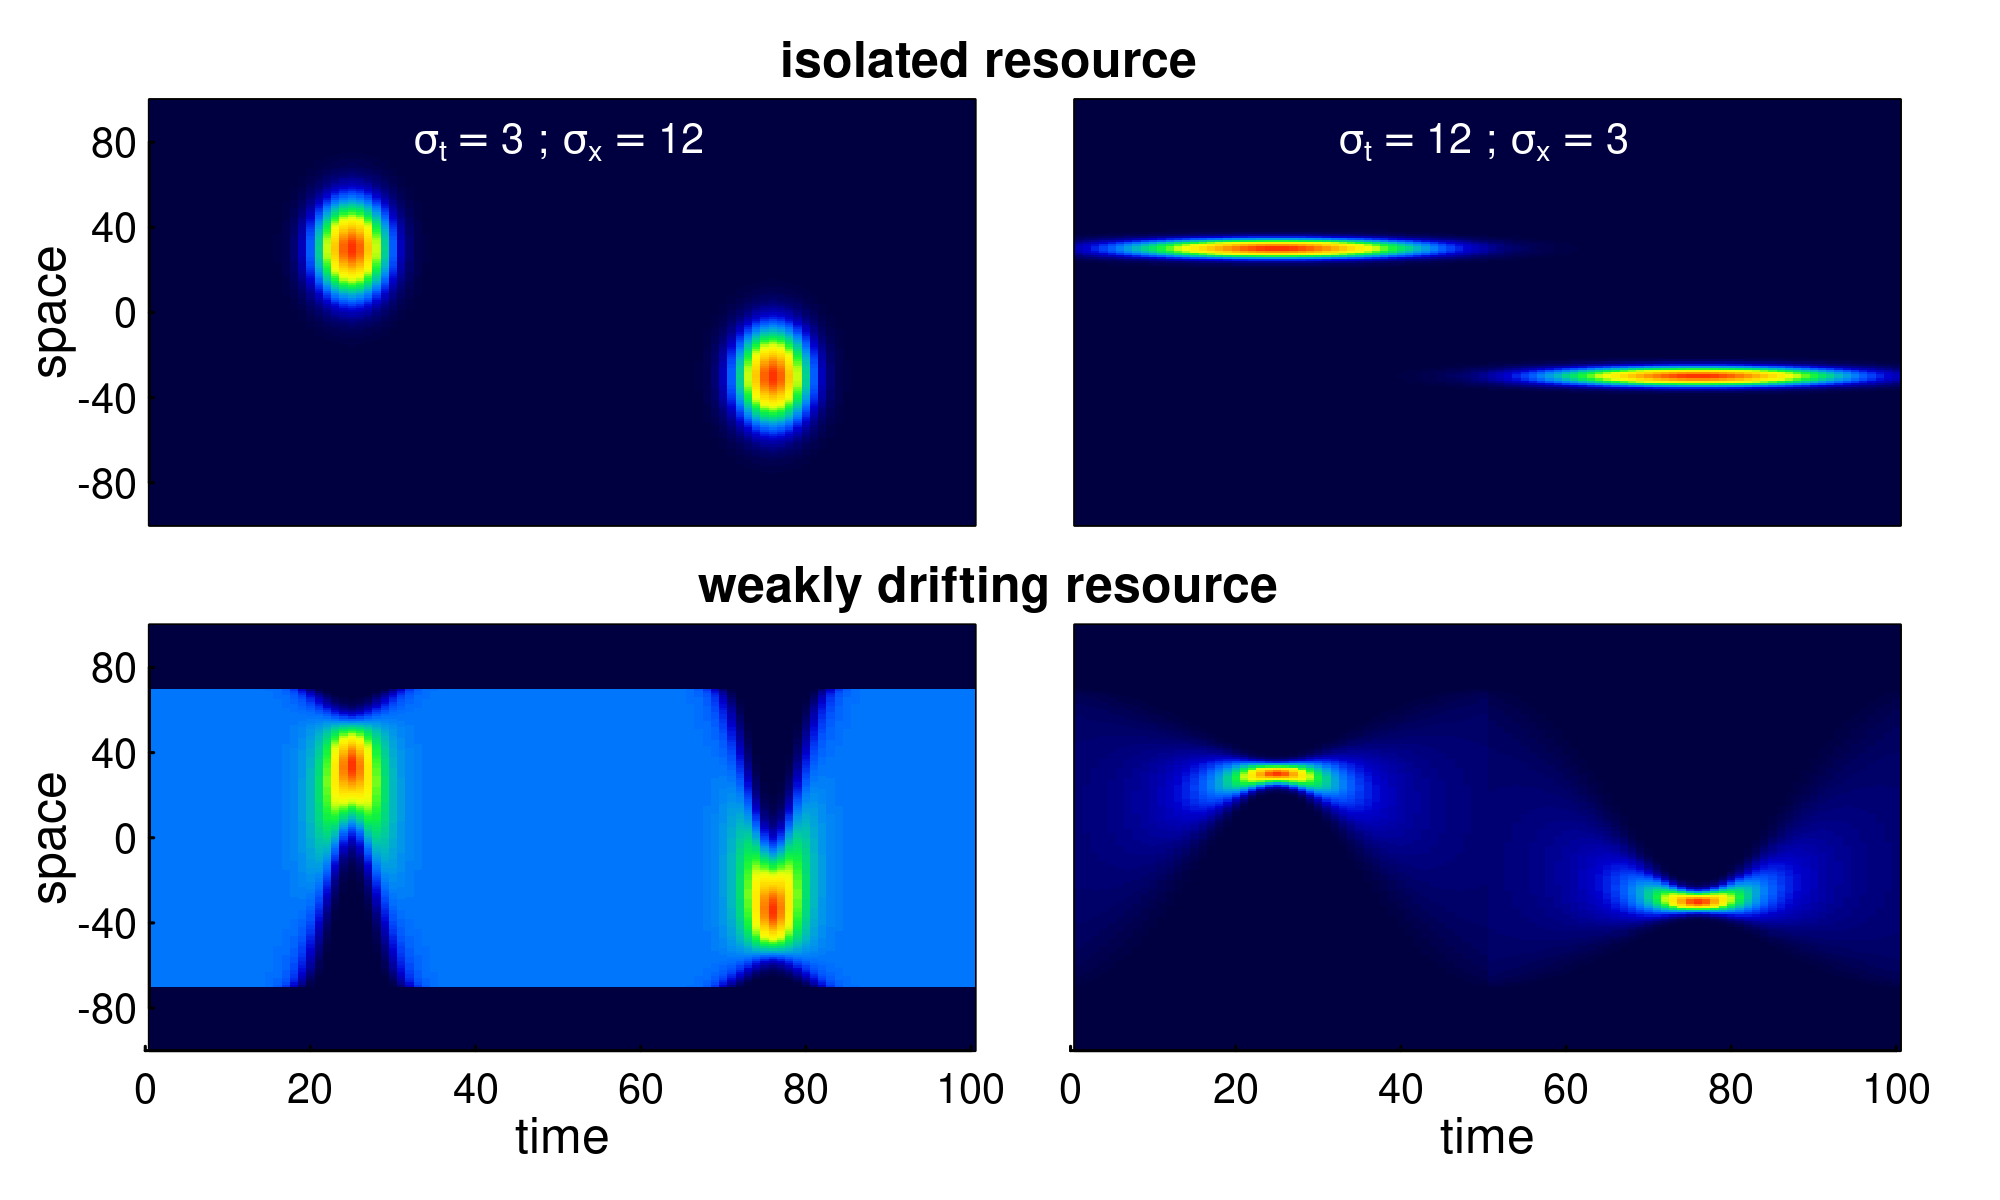
\includegraphics{figures/ResourceExamples.png}

\textbf{Figure 1. Examples of various seasonal resource distribution
functions, contrasting short duration, but wide pulses
(\(\sigma_t = 3, \sigma_x = 12\); left panels), long duration but
spatially concentrated pulses (\(\sigma_t = 12, \sigma_x = 3\); right
panels), and isolated resource pulses (upper panels) from the weakly
drifting resource (lower panels). The total amount of resource is
identical across all scenarios. In the weakly drifting resources, the
total amount is constant at all times, and uniform in the middle of the
phase (time = 0, 50, 100).}

\hypertarget{metrics}{%
\subsection{Metrics}\label{metrics}}

The main metrics we are interested in are \emph{migration mismatch},
\emph{foraging efficiency} and \emph{adaptation to trends}.

Migration mismatch captures the similarity between the migration
phenology and the resource phenology. To do this, we compute the total
mismatch, i.e.~is a sum of the difference between the migration
coefficients and the resource peaks. Thus, the spatial mismatch is given
by the absolute difference between the migration targets and the
resource peaks, i.e.~\(MM_x = |x_1 - m_x| + |x_2 + m_x|\). The temporal
mismatch is the difference between the arrival time and the peak of the
resource if arrival is post-peak, the difference between the departure
time and the peak of the resource if departure is pre-peak, and 0 if the
seasonal duration spans the peak,
i.e.~\(MM_t = max\{t_1 - m_1, m_1 - (t_1 + dt_1), 0\} + max\{t_2 - m_2, m_2 - (t_2 + dt_2), 0\}\).
The total mismatch is the sum of \(MM_x\) and \(MM_t\). A mismatch of
less than 1 is essentially perfect, we consider a mismatch of 1-5 to be
``good,'' and beyond 30 the system can be said to have failed to keep up
with climate change.

To quantify the foraging efficiency, i.e., the organisms' ability to
track the distribution of the resources over space and time, we use a
continuous form of the Bhattacharyya Coefficient (Bhattacharyya 1943)
which quantifies the similarity between two distributions. We compute
this coefficient at every time point in a given year, and take the mean
across the equilibrium year to determine foraging efficiency (FE). Thus,
the foraging efficiency index is:
$ FE = \frac{1}{\tau} \int_{0}^\tau \int_{-\chi}^{\chi} \sqrt{u(x,t) \, h(x,t)} \,\, dx\,dt\]
where the spatial integral is taken over the domain. This metric is
constrained to be between 0 and 1.

For simulations with a constant resource, we ran the model until a
quasi-equilibrium state was achieved, i.e.~where the Bhattacharya index
of the population distribution across subsequent years reached a value
of 0.9999. Once that state was attained, we computed the migration
mismatch and foraging efficiency metrics, as well as the number of years
required to reach stationarity.

For numerical runs with climate change, we first run a simulation for 20
years to attain an equilibrium, and then begin shifting the location of
the resource with a trend (slow 0.25, medium 0.5, or rapid 1 units per
year), or by adding stochasticity (s.d. 3, 6, 12). For the trend
analyses, we then compute the slope of the migration location parameter
against the resource drift and refer to this as the \emph{spatial
adaptation} (SA) index.

\hypertarget{simulation-studies}{%
\subsection{Simulation studies}\label{simulation-studies}}

We explored this model using numerical differencing of a system of
ordinary differential equations (ODE's) approximating the PDE in
equation (2) with the Runge-Kutte algorithm using the \texttt{deSolve}
(Soetaert et al. 2010) and \texttt{ReacTran} (Soetaert and Meysman 2012)
packages in R. We additionally used the \texttt{nlsLM} function in
package \texttt{minpack.LM} (Elzhov et al. 2016) for robust and fast
annual estimation of the migration parameters. The complete code is
available as an R package (\texttt{memorymigration}) available on GitHub
at \url{https://github.com/EliGurarie/memorymigration} and as an
interactive Shiny application at \url{https://url.to.be.determined}.

We assessed a wide range of parameter values and resource geometries and
dynamics with the goal of answering the four main questions: 1. Can this
model adapt to a discrete shift in peak resource location and timing?
What is the relative role of memory and sociality for adaptation? 2. Can
this model acquire a migratory behavior from a non-migratory initial
condition? 3. What is the role of a reference memory for dealing with
stochastic resource dynamics? 4. Can this model adapt when the resource
peaks shifts in space?

\textbf{Table 1} \emph{Parameters, variables and metrics.}

\begin{longtable}[]{@{}lll@{}}
\toprule
\begin{minipage}[b]{(\columnwidth - 2\tabcolsep) * \real{0.19}}\raggedright
\strut
\end{minipage} &
\begin{minipage}[b]{(\columnwidth - 2\tabcolsep) * \real{0.41}}\raggedright
Parameter\strut
\end{minipage} &
\begin{minipage}[b]{(\columnwidth - 2\tabcolsep) * \real{0.41}}\raggedright
Description\strut
\end{minipage}\tabularnewline
\midrule
\endhead
\begin{minipage}[t]{(\columnwidth - 2\tabcolsep) * \real{0.19}}\raggedright
\emph{Memory migration model}\strut
\end{minipage} &
\begin{minipage}[t]{(\columnwidth - 2\tabcolsep) * \real{0.41}}\raggedright
\strut
\end{minipage} &
\begin{minipage}[t]{(\columnwidth - 2\tabcolsep) * \real{0.41}}\raggedright
\strut
\end{minipage}\tabularnewline
\begin{minipage}[t]{(\columnwidth - 2\tabcolsep) * \real{0.19}}\raggedright
\strut
\end{minipage} &
\begin{minipage}[t]{(\columnwidth - 2\tabcolsep) * \real{0.41}}\raggedright
\(\epsilon\)\strut
\end{minipage} &
\begin{minipage}[t]{(\columnwidth - 2\tabcolsep) * \real{0.41}}\raggedright
Diffusion\strut
\end{minipage}\tabularnewline
\begin{minipage}[t]{(\columnwidth - 2\tabcolsep) * \real{0.19}}\raggedright
\strut
\end{minipage} &
\begin{minipage}[t]{(\columnwidth - 2\tabcolsep) * \real{0.41}}\raggedright
\(\alpha\)\strut
\end{minipage} &
\begin{minipage}[t]{(\columnwidth - 2\tabcolsep) * \real{0.41}}\raggedright
Forage following\strut
\end{minipage}\tabularnewline
\begin{minipage}[t]{(\columnwidth - 2\tabcolsep) * \real{0.19}}\raggedright
\strut
\end{minipage} &
\begin{minipage}[t]{(\columnwidth - 2\tabcolsep) * \real{0.41}}\raggedright
\(\beta\)\strut
\end{minipage} &
\begin{minipage}[t]{(\columnwidth - 2\tabcolsep) * \real{0.41}}\raggedright
Strength of sociality\strut
\end{minipage}\tabularnewline
\begin{minipage}[t]{(\columnwidth - 2\tabcolsep) * \real{0.19}}\raggedright
\strut
\end{minipage} &
\begin{minipage}[t]{(\columnwidth - 2\tabcolsep) * \real{0.41}}\raggedright
\(\lambda\)\strut
\end{minipage} &
\begin{minipage}[t]{(\columnwidth - 2\tabcolsep) * \real{0.41}}\raggedright
Spatial scale of sociality\strut
\end{minipage}\tabularnewline
\begin{minipage}[t]{(\columnwidth - 2\tabcolsep) * \real{0.19}}\raggedright
\strut
\end{minipage} &
\begin{minipage}[t]{(\columnwidth - 2\tabcolsep) * \real{0.41}}\raggedright
\(\kappa\)\strut
\end{minipage} &
\begin{minipage}[t]{(\columnwidth - 2\tabcolsep) * \real{0.41}}\raggedright
Proportion of reference versus working memory\strut
\end{minipage}\tabularnewline
\begin{minipage}[t]{(\columnwidth - 2\tabcolsep) * \real{0.19}}\raggedright
\strut
\end{minipage} &
\begin{minipage}[t]{(\columnwidth - 2\tabcolsep) * \real{0.41}}\raggedright
\(x_1\), \(x_2\)\strut
\end{minipage} &
\begin{minipage}[t]{(\columnwidth - 2\tabcolsep) * \real{0.41}}\raggedright
location of population centroids in summer and winter\strut
\end{minipage}\tabularnewline
\begin{minipage}[t]{(\columnwidth - 2\tabcolsep) * \real{0.19}}\raggedright
\strut
\end{minipage} &
\begin{minipage}[t]{(\columnwidth - 2\tabcolsep) * \real{0.41}}\raggedright
\(t_1\), \(dt_1\)\strut
\end{minipage} &
\begin{minipage}[t]{(\columnwidth - 2\tabcolsep) * \real{0.41}}\raggedright
start and duration of summer season\strut
\end{minipage}\tabularnewline
\begin{minipage}[t]{(\columnwidth - 2\tabcolsep) * \real{0.19}}\raggedright
\strut
\end{minipage} &
\begin{minipage}[t]{(\columnwidth - 2\tabcolsep) * \real{0.41}}\raggedright
\(t_2\), \(dt_2\)\strut
\end{minipage} &
\begin{minipage}[t]{(\columnwidth - 2\tabcolsep) * \real{0.41}}\raggedright
start and duration of winter season\strut
\end{minipage}\tabularnewline
\begin{minipage}[t]{(\columnwidth - 2\tabcolsep) * \real{0.19}}\raggedright
\strut
\end{minipage} &
\begin{minipage}[t]{(\columnwidth - 2\tabcolsep) * \real{0.41}}\raggedright
\(\kappa\)\strut
\end{minipage} &
\begin{minipage}[t]{(\columnwidth - 2\tabcolsep) * \real{0.41}}\raggedright
proportion memory allocated to reference (long-term) memory
vs.~short-term memory\strut
\end{minipage}\tabularnewline
\begin{minipage}[t]{(\columnwidth - 2\tabcolsep) * \real{0.19}}\raggedright
\emph{Resource dynamics}\strut
\end{minipage} &
\begin{minipage}[t]{(\columnwidth - 2\tabcolsep) * \real{0.41}}\raggedright
\strut
\end{minipage} &
\begin{minipage}[t]{(\columnwidth - 2\tabcolsep) * \real{0.41}}\raggedright
\strut
\end{minipage}\tabularnewline
\begin{minipage}[t]{(\columnwidth - 2\tabcolsep) * \real{0.19}}\raggedright
\strut
\end{minipage} &
\begin{minipage}[t]{(\columnwidth - 2\tabcolsep) * \real{0.41}}\raggedright
\(\tau\)\strut
\end{minipage} &
\begin{minipage}[t]{(\columnwidth - 2\tabcolsep) * \real{0.41}}\raggedright
duration of period (year)\strut
\end{minipage}\tabularnewline
\begin{minipage}[t]{(\columnwidth - 2\tabcolsep) * \real{0.19}}\raggedright
\strut
\end{minipage} &
\begin{minipage}[t]{(\columnwidth - 2\tabcolsep) * \real{0.41}}\raggedright
\(m_x\), \(-m_x\)\strut
\end{minipage} &
\begin{minipage}[t]{(\columnwidth - 2\tabcolsep) * \real{0.41}}\raggedright
spatial coordinate of resource peak for summer and winter\strut
\end{minipage}\tabularnewline
\begin{minipage}[t]{(\columnwidth - 2\tabcolsep) * \real{0.19}}\raggedright
\strut
\end{minipage} &
\begin{minipage}[t]{(\columnwidth - 2\tabcolsep) * \real{0.41}}\raggedright
\(m_t\), \(\tau - m_t\)\strut
\end{minipage} &
\begin{minipage}[t]{(\columnwidth - 2\tabcolsep) * \real{0.41}}\raggedright
timing of resource peak for the summer and winter\strut
\end{minipage}\tabularnewline
\begin{minipage}[t]{(\columnwidth - 2\tabcolsep) * \real{0.19}}\raggedright
\strut
\end{minipage} &
\begin{minipage}[t]{(\columnwidth - 2\tabcolsep) * \real{0.41}}\raggedright
\(\sigma_x\), \(\sigma_t\)\strut
\end{minipage} &
\begin{minipage}[t]{(\columnwidth - 2\tabcolsep) * \real{0.41}}\raggedright
time duration and and spatial scale of resource pulse\strut
\end{minipage}\tabularnewline
\begin{minipage}[t]{(\columnwidth - 2\tabcolsep) * \real{0.19}}\raggedright
\strut
\end{minipage} &
\begin{minipage}[t]{(\columnwidth - 2\tabcolsep) * \real{0.41}}\raggedright
\(dx\), \(dt\)\strut
\end{minipage} &
\begin{minipage}[t]{(\columnwidth - 2\tabcolsep) * \real{0.41}}\raggedright
rate of change of peak locaton and timing of resource\strut
\end{minipage}\tabularnewline
\begin{minipage}[t]{(\columnwidth - 2\tabcolsep) * \real{0.19}}\raggedright
\strut
\end{minipage} &
\begin{minipage}[t]{(\columnwidth - 2\tabcolsep) * \real{0.41}}\raggedright
\(\psi_x\), \(\psi_t\)\strut
\end{minipage} &
\begin{minipage}[t]{(\columnwidth - 2\tabcolsep) * \real{0.41}}\raggedright
standard deviation of peak location and timing\strut
\end{minipage}\tabularnewline
\begin{minipage}[t]{(\columnwidth - 2\tabcolsep) * \real{0.19}}\raggedright
\emph{Metrics}\strut
\end{minipage} &
\begin{minipage}[t]{(\columnwidth - 2\tabcolsep) * \real{0.41}}\raggedright
\strut
\end{minipage} &
\begin{minipage}[t]{(\columnwidth - 2\tabcolsep) * \real{0.41}}\raggedright
\strut
\end{minipage}\tabularnewline
\begin{minipage}[t]{(\columnwidth - 2\tabcolsep) * \real{0.19}}\raggedright
\strut
\end{minipage} &
\begin{minipage}[t]{(\columnwidth - 2\tabcolsep) * \real{0.41}}\raggedright
\(MM_x\)\strut
\end{minipage} &
\begin{minipage}[t]{(\columnwidth - 2\tabcolsep) * \real{0.41}}\raggedright
spatial migration mismatch\strut
\end{minipage}\tabularnewline
\begin{minipage}[t]{(\columnwidth - 2\tabcolsep) * \real{0.19}}\raggedright
\strut
\end{minipage} &
\begin{minipage}[t]{(\columnwidth - 2\tabcolsep) * \real{0.41}}\raggedright
\(MM_t\)\strut
\end{minipage} &
\begin{minipage}[t]{(\columnwidth - 2\tabcolsep) * \real{0.41}}\raggedright
temporal migration mismatch\strut
\end{minipage}\tabularnewline
\begin{minipage}[t]{(\columnwidth - 2\tabcolsep) * \real{0.19}}\raggedright
\strut
\end{minipage} &
\begin{minipage}[t]{(\columnwidth - 2\tabcolsep) * \real{0.41}}\raggedright
\(TE\)\strut
\end{minipage} &
\begin{minipage}[t]{(\columnwidth - 2\tabcolsep) * \real{0.41}}\raggedright
total mismatch\strut
\end{minipage}\tabularnewline
\begin{minipage}[t]{(\columnwidth - 2\tabcolsep) * \real{0.19}}\raggedright
\strut
\end{minipage} &
\begin{minipage}[t]{(\columnwidth - 2\tabcolsep) * \real{0.41}}\raggedright
\(FE\)\strut
\end{minipage} &
\begin{minipage}[t]{(\columnwidth - 2\tabcolsep) * \real{0.41}}\raggedright
foraging efficiency\strut
\end{minipage}\tabularnewline
\begin{minipage}[t]{(\columnwidth - 2\tabcolsep) * \real{0.19}}\raggedright
\strut
\end{minipage} &
\begin{minipage}[t]{(\columnwidth - 2\tabcolsep) * \real{0.41}}\raggedright
\(SA\)\strut
\end{minipage} &
\begin{minipage}[t]{(\columnwidth - 2\tabcolsep) * \real{0.41}}\raggedright
spatial adaptation index\strut
\end{minipage}\tabularnewline
\bottomrule
\end{longtable}

\hypertarget{results}{%
\section{Results}\label{results}}

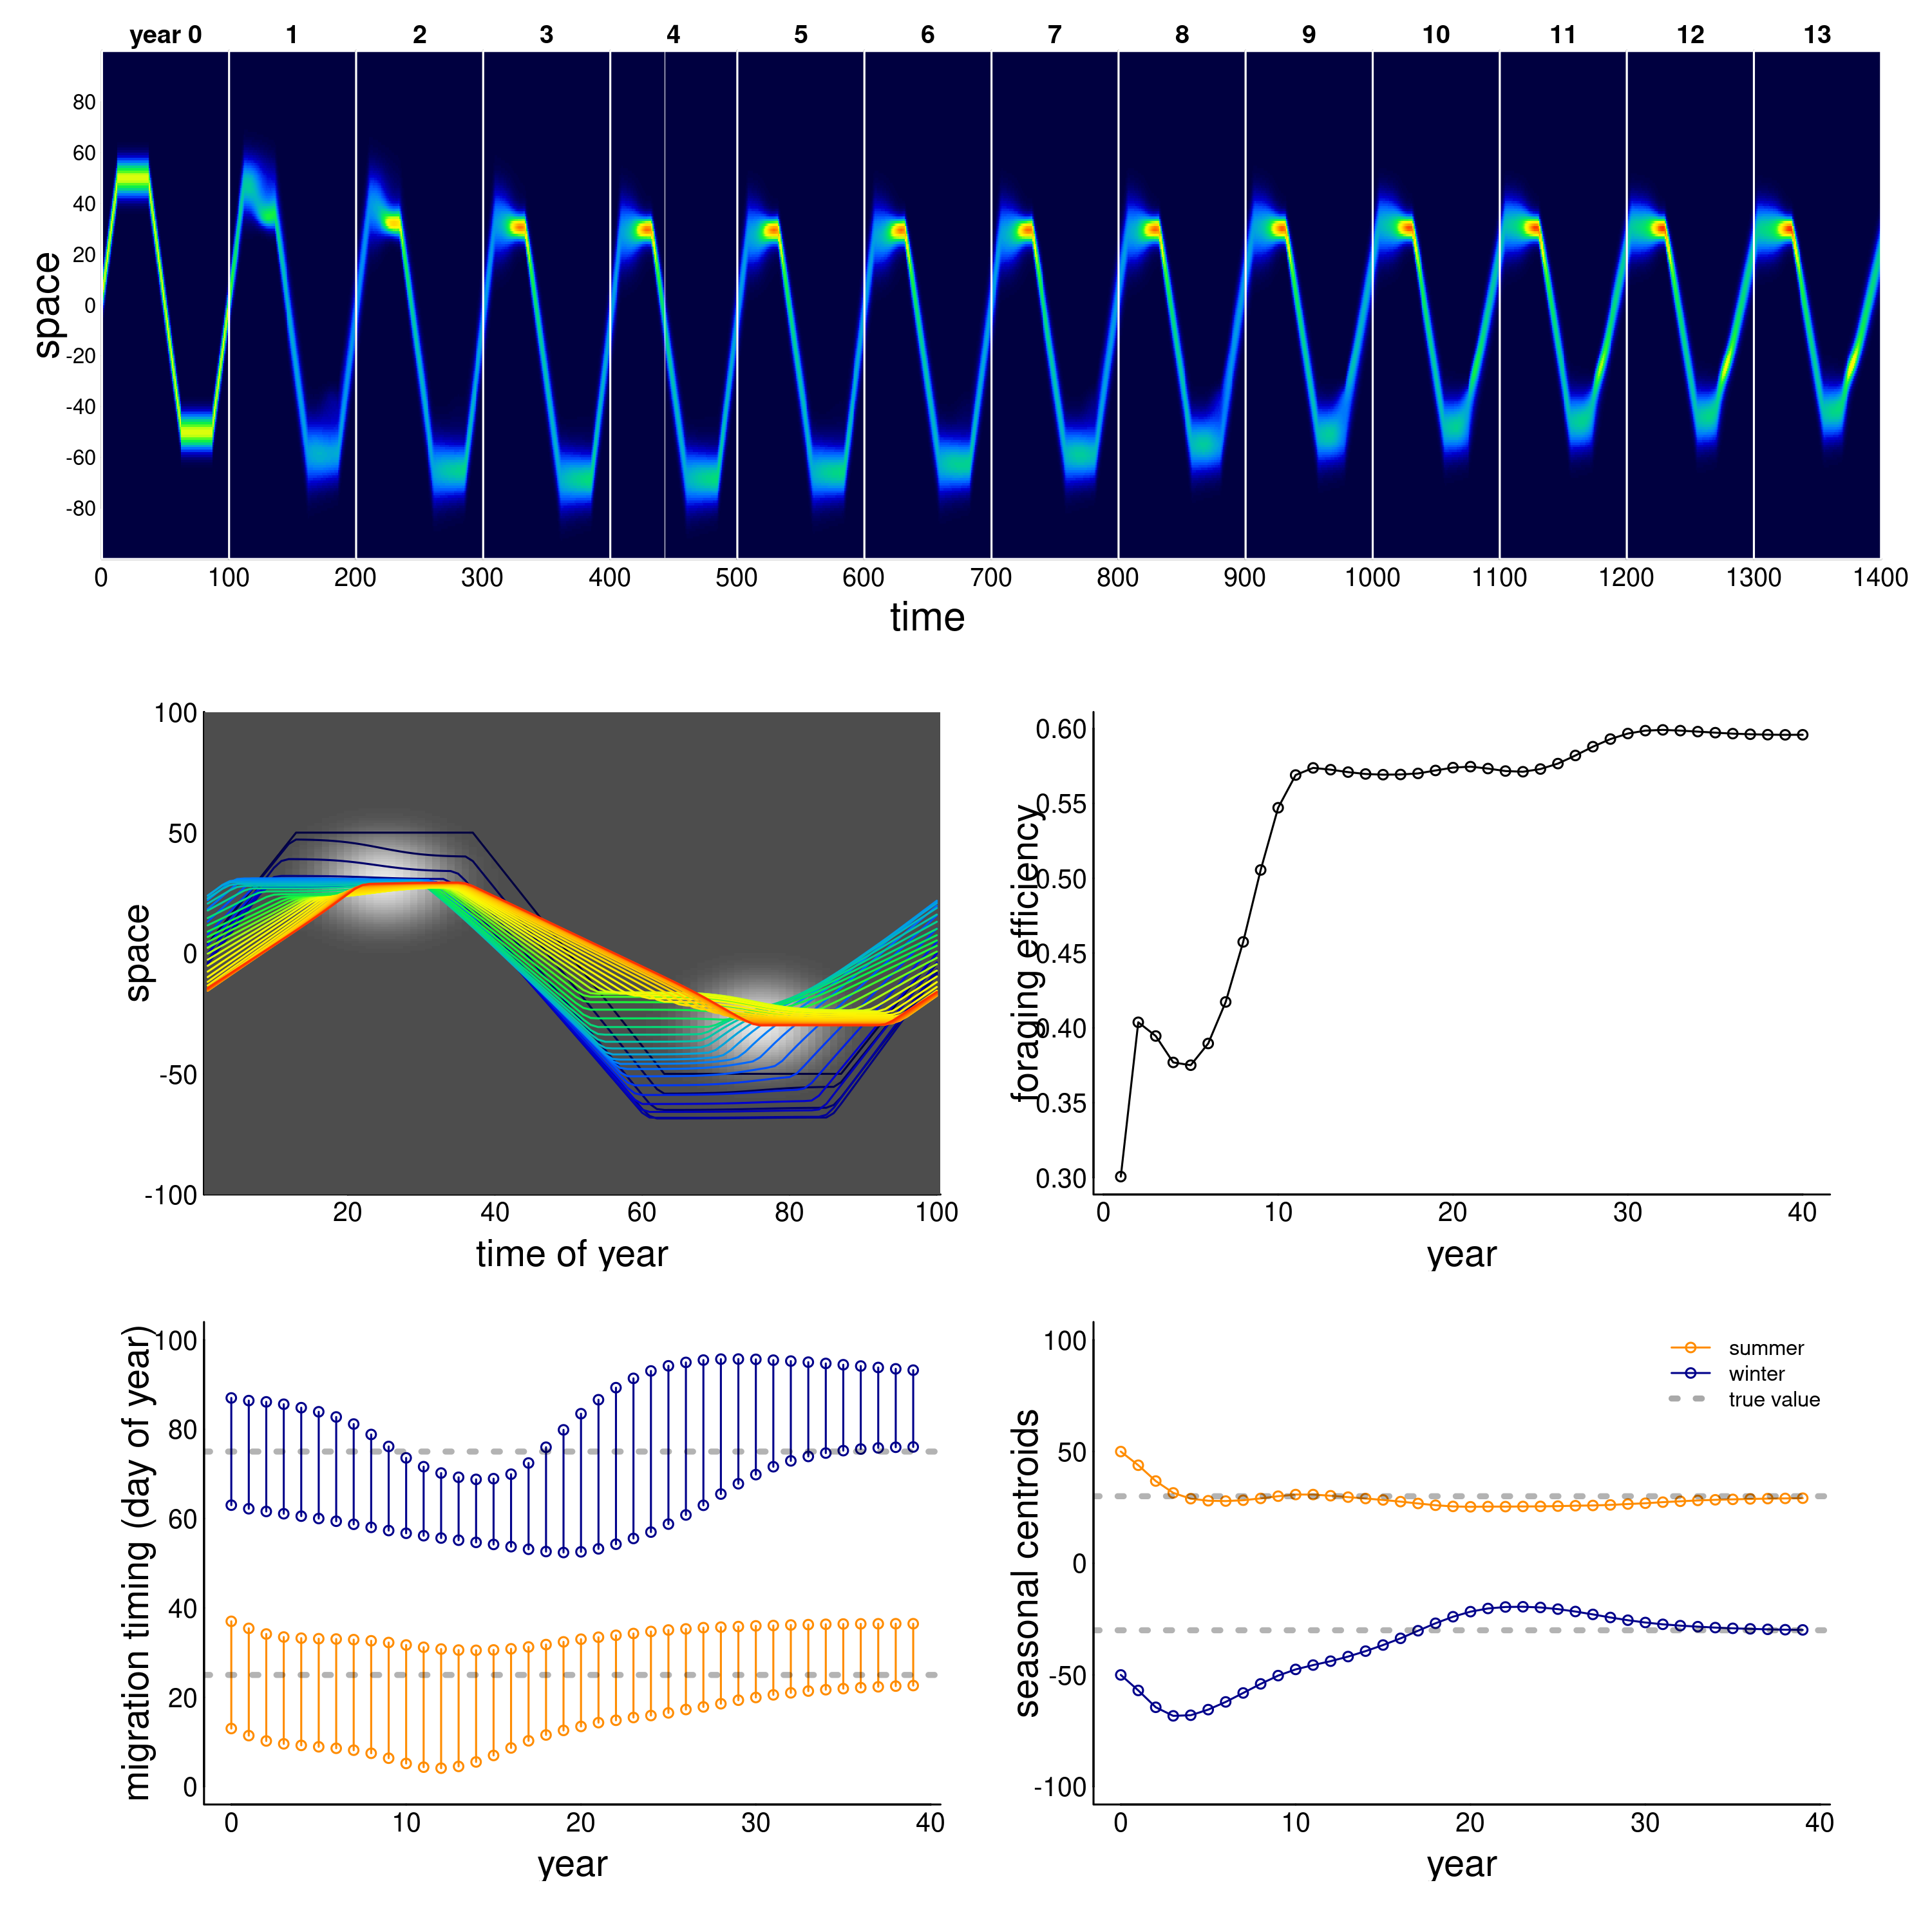
\includegraphics{figures/example1_adaptation.png}

\textbf{Figure 2.} \emph{Example of adaptation to a shift in resource
peak. The initial (year 0) behavior migrates to locations 50 and -50 at
days 15 and 60, whereas the resource peak is at 30 and -30, peaking at
times 25 and 75. The panels show (a) the first 14 years of the
simulation; (b) the centroid of the annual movement of the population is
shown in panel b, with dark blue to red colors indicating year 0 to year
40; (c) annual foraging efficiency across years; (d) migration timing
parameters for each year, with orange segments indicating arrival and
departure from the summering (northern) grounds, and the blue segments
indicating timing of arrival and departure at the wintering grounds; (e)
migration arrival and departure location across years, with blue and
orange indicating winter (southern) and summer (northern) locations.}

\hypertarget{adaptation-to-resource-phenology}{%
\subsection{Adaptation to resource
phenology}\label{adaptation-to-resource-phenology}}

The ability of this system to attain stable, migratory state that
matches the dynamics of the resource is illustrated in Figure 2. In the
illustrated scenario, it takes nearly 40 years to attain an equilibrium,
and the eventual steady state is one where the centroid of the migration
lines up exactly with the centroid of the resource, and the arrival
timing coincides with the \emph{peak} of resource availability. Notably,
the path to this equilibrium is somewhat indirect, with the later winter
range taking more time to stabilize than the earlier summer range. The
eventual steady state is one where the foraging efficiency is relatively
high.

We ran this process for 8100 parameter combinations (Figure 3). The
fundamental dynamic of attaining and maintaining a well-matched
migration phenology, can occur under many combinations of parameter
values, but all parameters play a role. Among the more intuitive results
are that greater values of \(\alpha\) (resource following) lead to an
improved ability to match the migration. Resource peaks with larger
spatial extent (higher \(\sigma_x\)) are generally better for migration
matching. A larger set of parameters matched migration with low
diffusion than high diffusion.

Less intuitive was the high importance of the sociality parameters, in
particular the spatial scale of the swarming. Higher levels of social
attraction (\(\beta\)) led to improved migration matching except in
those cases where the sociality scale \(\lambda\) was high. Thus, for
example, at \(\lambda = 20\), no simulations at \(\beta >= 200\) managed
to acquire or maintain a matched migration. However, at \(\lambda = 50\)
or \(100\), the migration was slightly better matched at high values of
\(\beta\). (Fig. \textbf{X}) The spatial extent of the swarm was a
remarkably significant variable. Smaller swarms were able to match
migration only at low values of social attraction (\(\beta = 200\)), and
relatively high values of resource attraction (\(\alpha \geq 600\)).

Random forest analyses, whether on the log of total mismatch or on the
classification of a perfect match, uniformly show that the most
important variables (Breiman 2001) were \(\alpha\) and \(\lambda\) (4.14
and 4.02 proportional increase in MSE), and the least important was
\(\sigma_t\), with a 0.5 proportional increase (table \textbf{X}).

Overall, foraging efficiency was strongly correlated with migration
matching, as expected. At high mismatch (\textgreater{} 50), foraging
efficiency was low (mean 0.29, s.d. 0.16) compared to the near-perfect
matching migrations (mean 0.58, s.d. 0.14). However, somewhat higher
mismatch (1 to 5) showed an even higher overall foraging efficiency
(mean 0.62, s.d. 0.18 - see also Figure \textbf{X}).

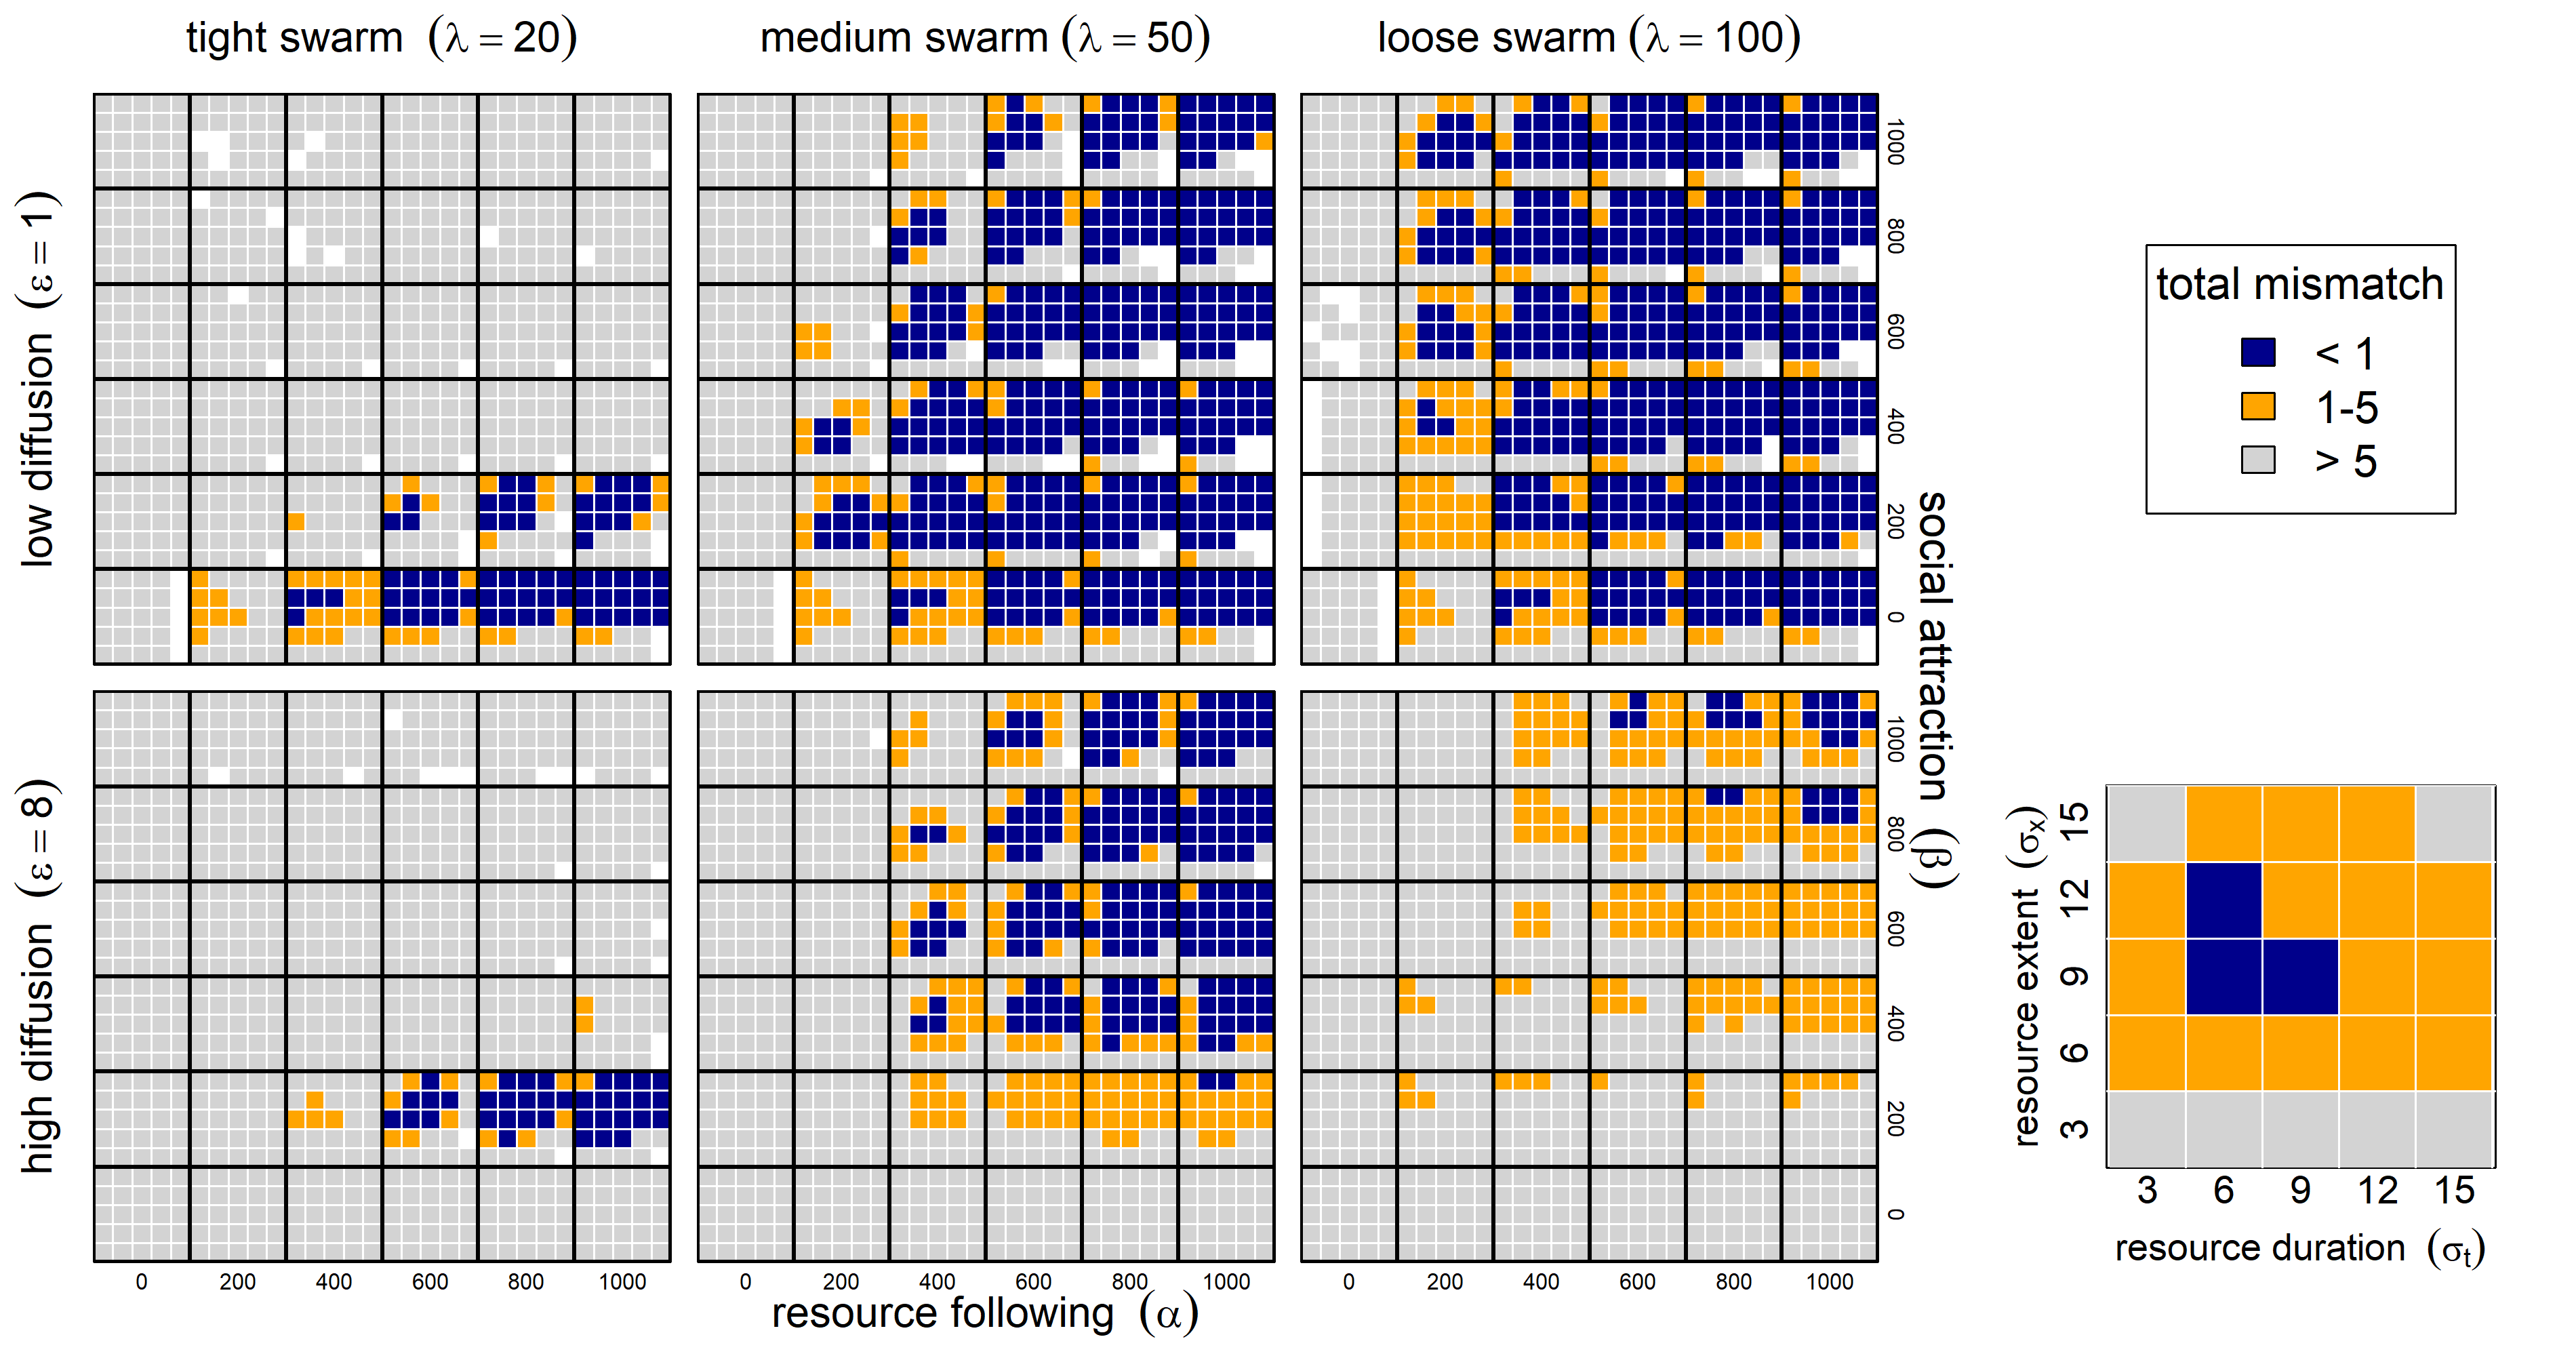
\includegraphics{figures/StabilityResults.png} \textbf{Figure 3.}
\emph{Migration phenology matching across six model parameters. Low and
high diffusion (\(\epsilon = 1\) and \(8\) in upper and lower panel
blocks), tight, medium and loose swarms (\(\lambda = 20, 50, 100\)) left
to right panels. Within each of these blocks, high values of the
resource following parmaeters \(\alpha\) from 0 to 1000 are left to
right, and higher values of the sociality parameter \(\beta\) are bottom
to top. Within each of the combinations of
\(\epsilon, \lambda, \alpha, \beta\), we show results ranging across 6
values of resource duration (\(\sigma_t\), 3-15 left to right), and 6
values of resource extent (\(\sigma_x\), 3-15 bottom to top), as in the
zoomed in panel at bottom right. The color scheme reflects the total
mismatch, i.e.~the sum of the absolute differences between the migration
timing and locations from the resource peak. White squares represent
runs that numerically failed to estimate migration parameters.}

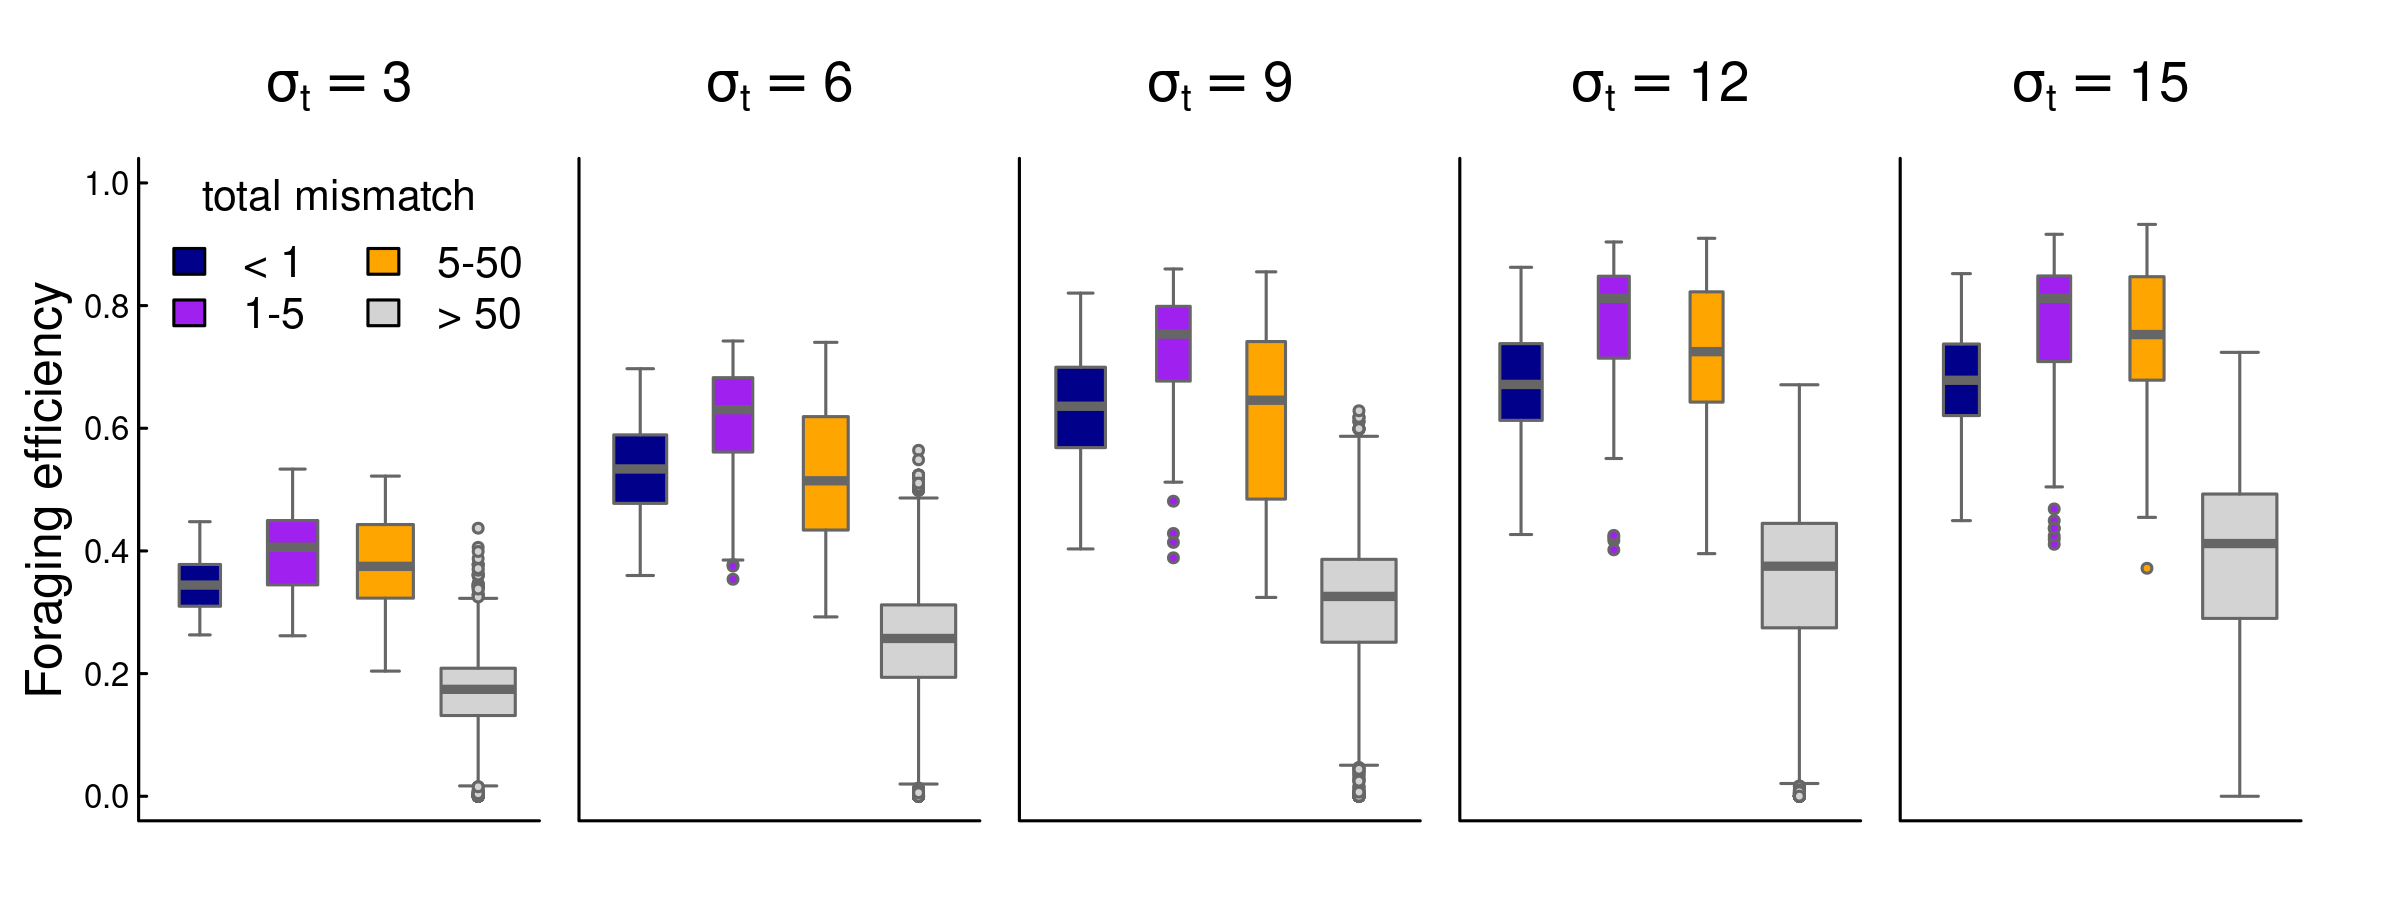
\includegraphics{figures/ForagingEfficiency.png}

\textbf{Figure 4.} \emph{Box-plots of foraging efficiency against
mismatch across several values of foraging patch duration.}

\hypertarget{learning-to-migrate}{%
\subsection{Learning to migrate}\label{learning-to-migrate}}

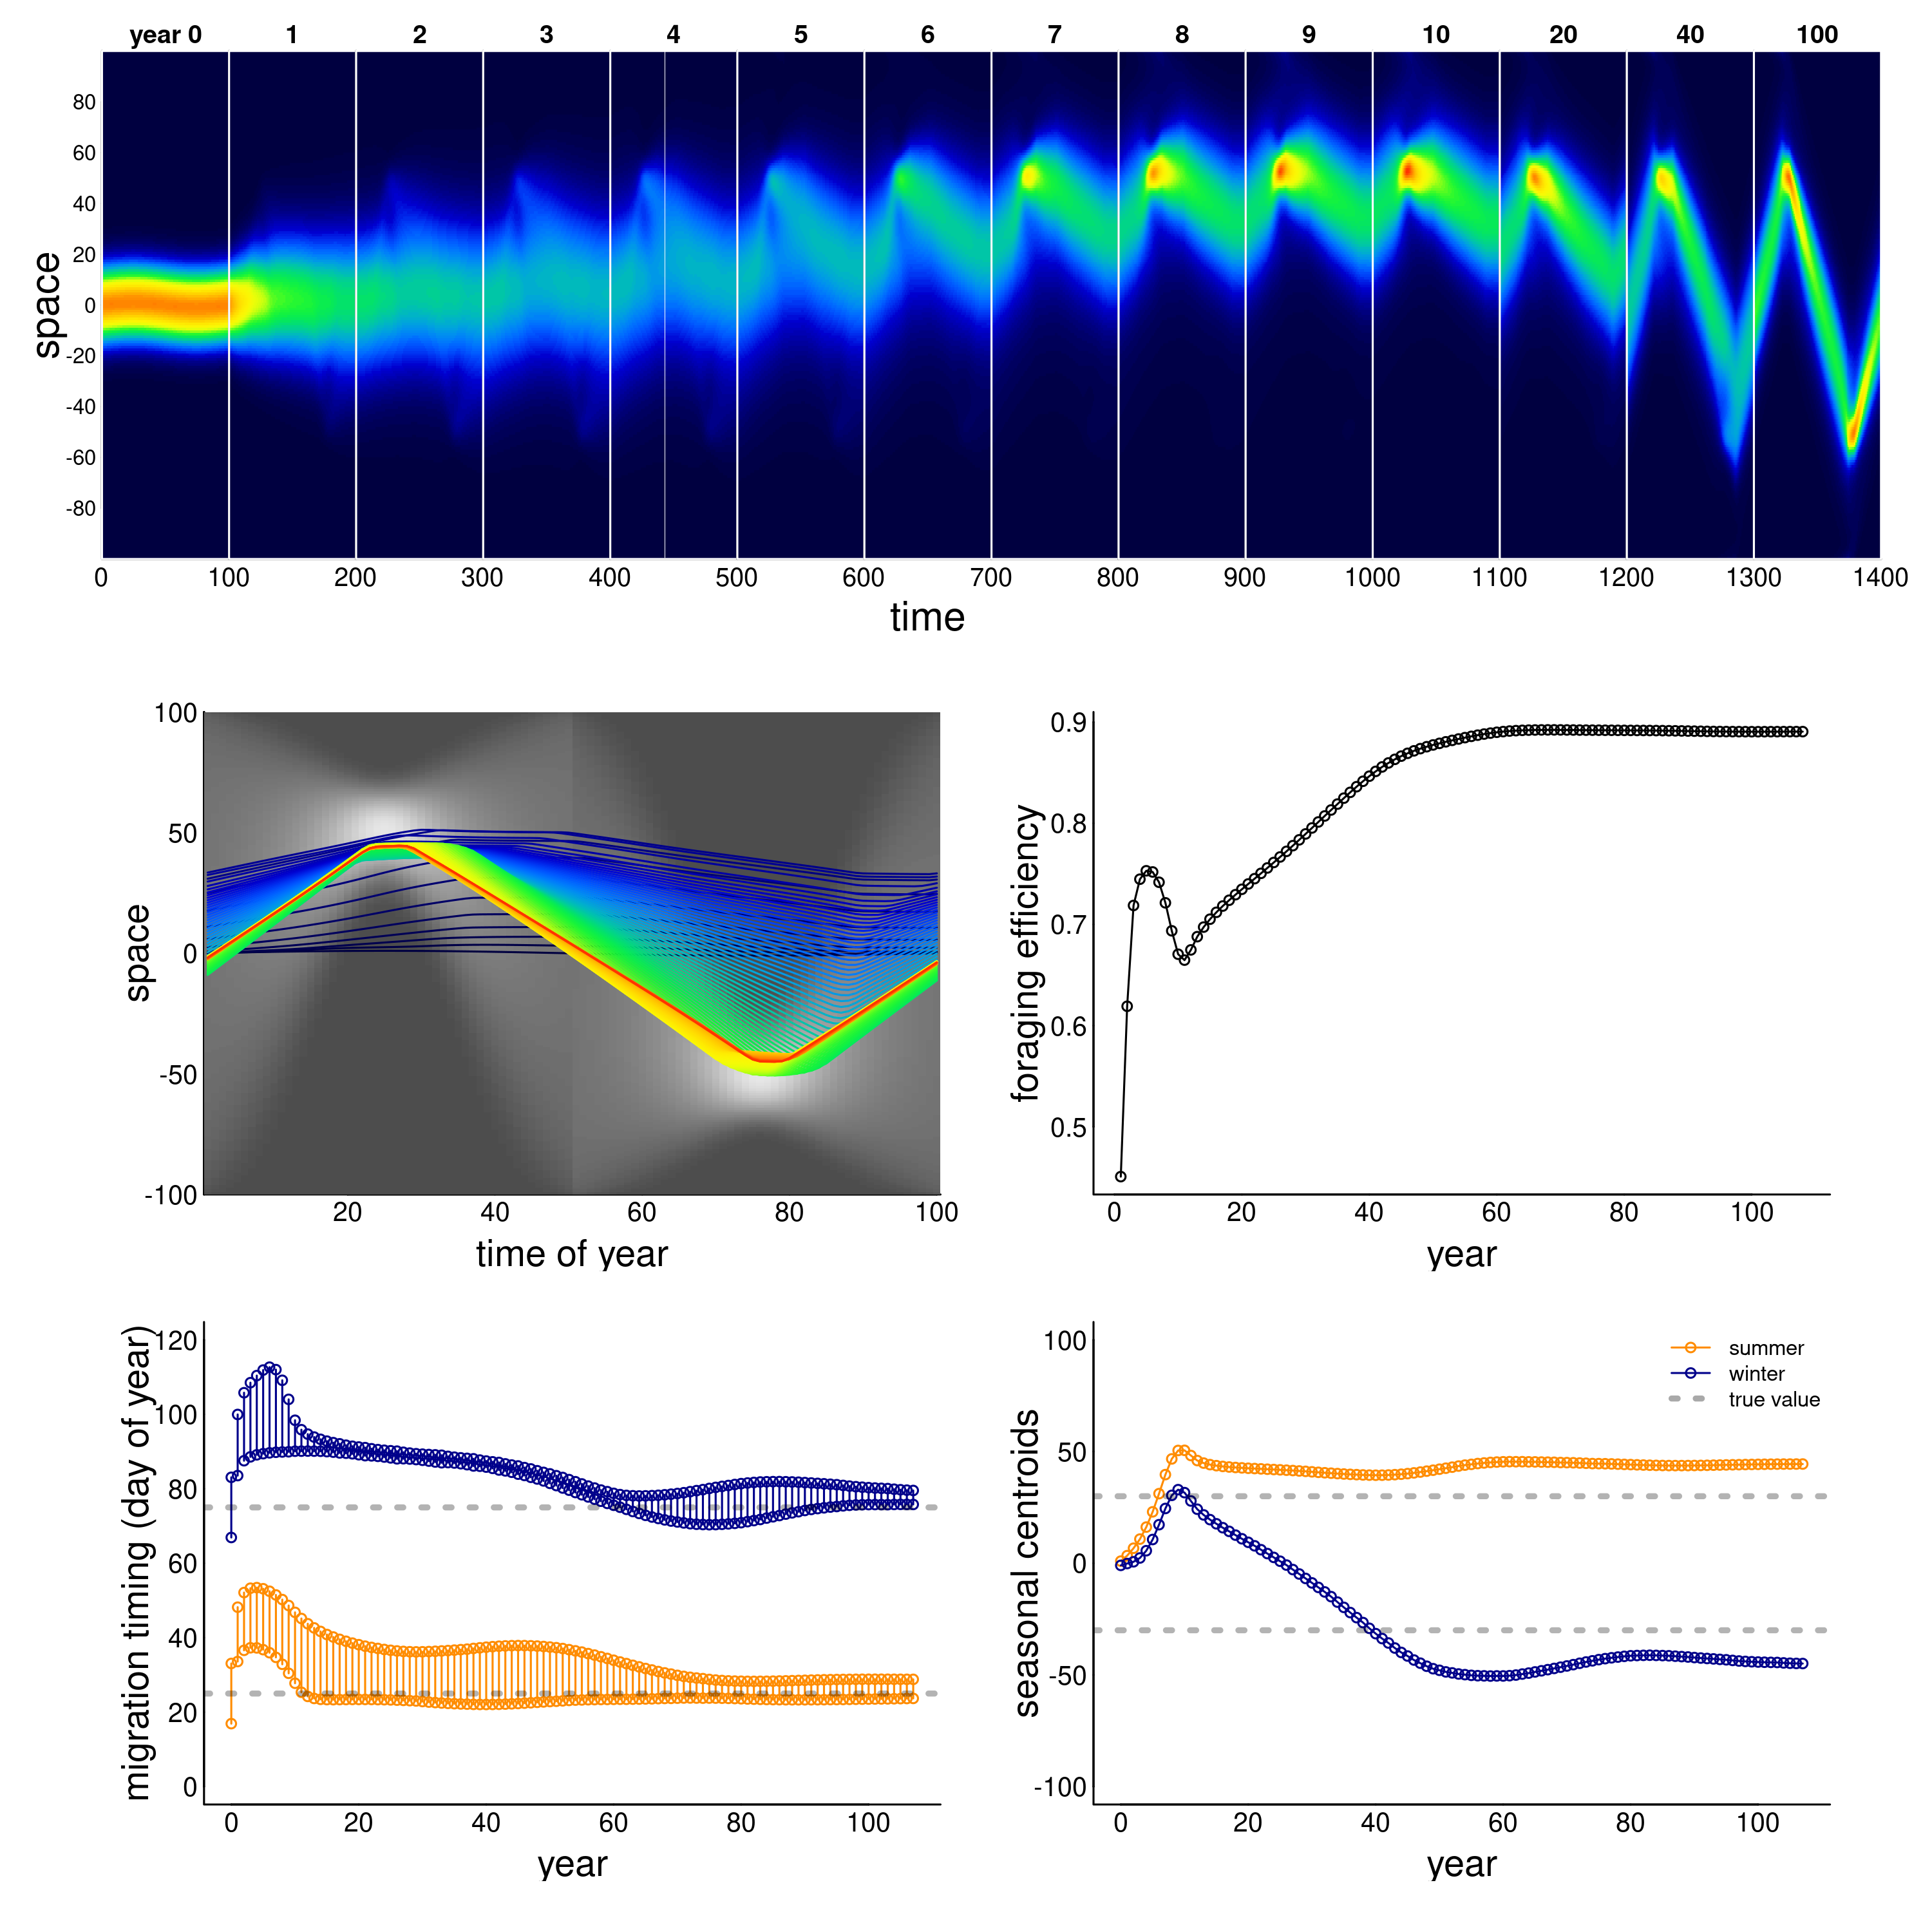
\includegraphics{figures/example2_learningtomigrate.png} \textbf{Figure
5.} \emph{Example of model learning to migrate. The resource is a
``weakly drifting'' resource and the initial (year 0) condition is non
migratory. The simulation was run for 100 years, and a sampling of those
years (labeled) are presented in panel a: all years from 0 to 10,
followerd by 20, 40 and 100. Otherwise, panels are as in Figure 1.
Parameter values were \(\epsilon = 5\), \(\alpha = 500\) and
\(\beta = 50\).}

Figure \textbf{5} illustrates the ability of the model animals to learn
to migrate in a weakly drifting resource environment with a narrow pulse
of resource peaking at 30 and -30 (at days 25 and 75), but a uniform
distribution of resource at times 0 and 50. In order to learn to
migrate, the system needed to have a higher exploratory impulse (higher
diffusion constant \(\epsilon\)), a stronger resource advection (higher
\(\alpha\)) and somewhat weaker sociality (lower \(\beta\)). The
qualitative behavior of this process was to start drifting towards the
summer resource, while slowly developing a weak pulse towards the winter
resource as well. After first locking in on the summer resource, the
winter migration, driven both by high diffusion and high resource
following, slowly extended itself until both narrow peaks of resource
can be consistently reached.

The model had, in general, a difficult time learning migration from a
non-migratory initial condition. Thus, out of 4047 successful runs, only
4 attained mismatch below 1, and 130 below 5. Conditions that were more
conducive to learning migration were pulses of \emph{longer} duration
(high \(\sigma_t\)), but \emph{smaller} in scope (low \(\sigma_x\)),
suggesting that the feedback that encourages migration needs to be
compact in space but long enough in duration to lock in to the memory.

\hypertarget{adapting-to-climate-change}{%
\subsection{Adapting to climate
change}\label{adapting-to-climate-change}}

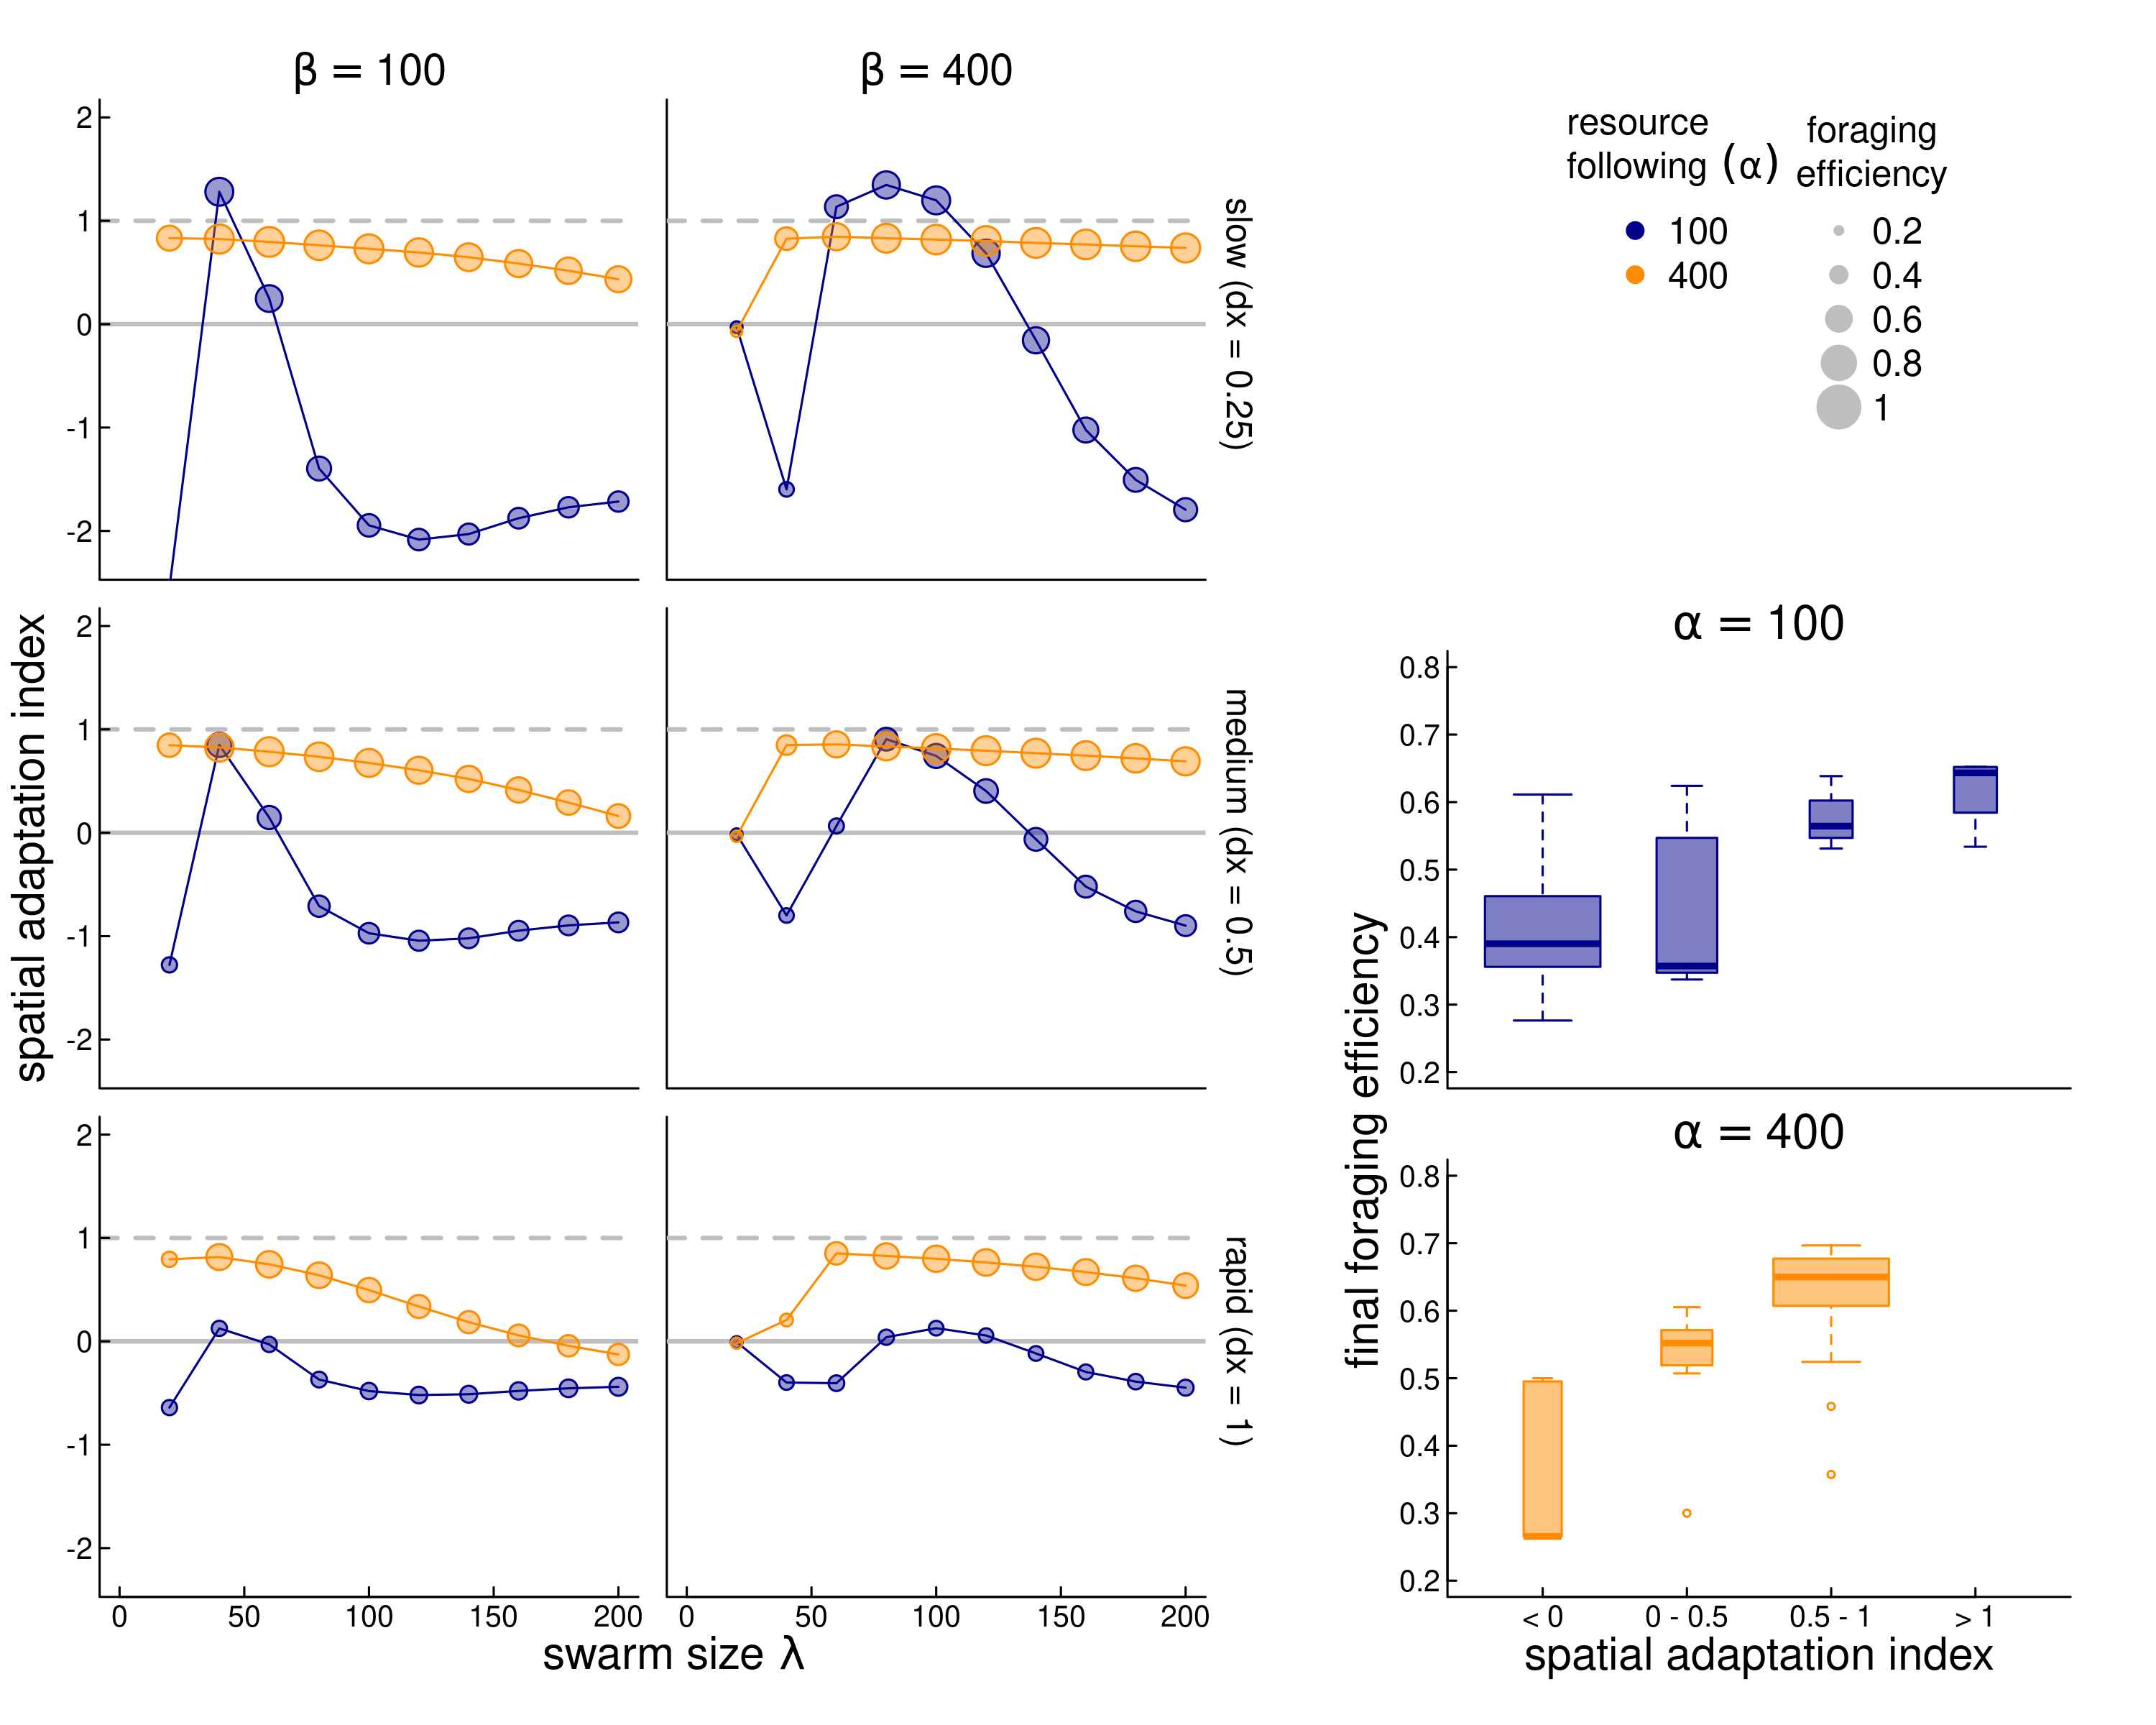
\includegraphics{figures/SpatialClimateChange.png}

\textbf{Figure 6.} \emph{Adaptation to a steadily drifting resource. In
three scenarios, the spatial coordinates of the resource drift by 0.25,
0.5, and 1 unit per year (top to bottom, respectively). The y-axis is
the index of spatial adaptation (SA), i.e.~the trend of the
memory-driven migration divided by the resource drift trend. Values near
1 indicate a behavior that keeps up with climate change, values near
indicate no change in migration behavior, and negative values indicate a
trend that is opposite to the climate trend. We compare across spatial
scales of sociality (\(\lambda\) - x-axis), for low and high values
resource following (\(\alpha = 400\) and \(100\) - orange and blue dots)
and low and high values of sociality (\(\beta = 100\) and 400, left and
right panels). The size of the circles is proportional to the foraging
efficiency of the resulting parameter combinations. The bottom-right
boxplots indicate the final year foraging efficiency against the SA
index; purple and blue boxes indicate the highest values, orange and
gray lower values.}

To assess the ability of the system to adapt to a trending climate, we
generated scenarios with slow (0.25 units / year), medium (0.5 units /
year), and fast (1 unit / year) drift outward of the two resource
pulses. We then assessed 40 parameter combinations for each of those
scenarios, a high and low value of resource following (\(\alpha = 400\)
and \(100\)) crossed with a high and low value of sociality
(\(\beta = 400\) and \(100\)) crossed with 10 values of the spatial
scale of sociality (\(\lambda = 20\) to \(200\)). The spatial and
temporal scale of the resource pulses were fixed to a relatively
``easy'' to adapt to \(\sigma_x = 12\) and \(\sigma_t = 6\). We computed
the adaptation index and foraging efficiency for each of the 120 runs
(figure \textbf{Z}). We were interested in the dynamics against
\(\lambda\) due to the uniformly high importance of this parameter for
determining the success of this process to match migration in steady
states.

As figure 6 shows, higher values of resource following
(\(\alpha = 400\); orange circles) are nearly universally better for
keeping up with climate change (SA values near 1). Furthermore, when
combined with high sociality (\(\beta = 400\); right panels), nearly all
parameter combinations do a good job keeping up with climate change (SA
values ranging between 0.53 and 0.85 for a swarm size greater than 50).
However, that maximum value is still less than 1, suggesting that truly
matching a steadily drifting trend is very difficult. Small swarms
(\(\lambda < 50\)) have a very hard time adapting when the social
attraction is high, but do fairly well when social attraction is lower.
But larger sized swarms do progressively worse across more
parameterizations, e.g.~in the most rapid climate change scenario, the
SA drops from 0.83 to -0.13 as the swarm increases in size from 40 to
200 (essentially, the entire spatial domain).

A rather more dramatic pattern is visible for the lower foraging
attraction scenario (\(\alpha = 100\); blue circles). Notably, no
parameter combination at this value comes close to keeping up with the
rapid climate change (SA range -0.64 to 0.13). For slower climate
change, however, there is a window of values for the swarm size -
relatively small, between 40 and 80, where the SA \emph{exceeds} 1, and
then crashing quite rapidly to negative values of SA as that swarm size
increases. These ``super-adapting'' processes indicate a unique sweet
spot where a swarm is large enough to capture and adapt to the drifting
resource, but not so large that the information gathered in a given year
is too weak to adjust the migratory behavior in a following year.

As anticipated, better adaptation to the drifting resource correlated
strongly with higher foraging efficiency (inset boxplots).

\hypertarget{reference-memory-and-stochasticity}{%
\subsection{Reference memory and
stochasticity}\label{reference-memory-and-stochasticity}}

While recent memory can be helpful for adapting to a single novelty or a
smoothly changing conditions, we hypothesized that more conservative
approach, relying on a ``reference memory'' may be more beneficial when
conditions change stochastically. We tested this hypothesis by solving a
set of models across a range of \(\kappa\) values fom 0 (all recent
memory) to 1 (all reference memory). In these scenarios, we ran the
system for as many years as needed with no stochasticity to acquire a
stationary state (i.e.~similarity index greater than 1-1e-6). We then
used the stationary state as the reference memory, and then ran the
process for an additional 50 years with a stochasticity (i.e.~standard
deviation in peak location of the resource) ranging from 0 to 12.

Figure 7 illustrates that, as predicted, the highest level of \(\kappa\)
can significantly help foraging efficiency; however this is highly
sensitive to the spatial scale of sociality. When that scale of
sociality is high enough (e..g \(\lambda = 120\), blue colors) there is
greater probability of overlap with a stochastic resource, and a
conservative, stable migratory regime is much more beneficial in the
long run. Overall, as anticipated, the greater the stochasticity, the
lower the foraging efficiency; and the greater the stochasticity, the
greater the benefit of a conservative reference memory driven strategy.

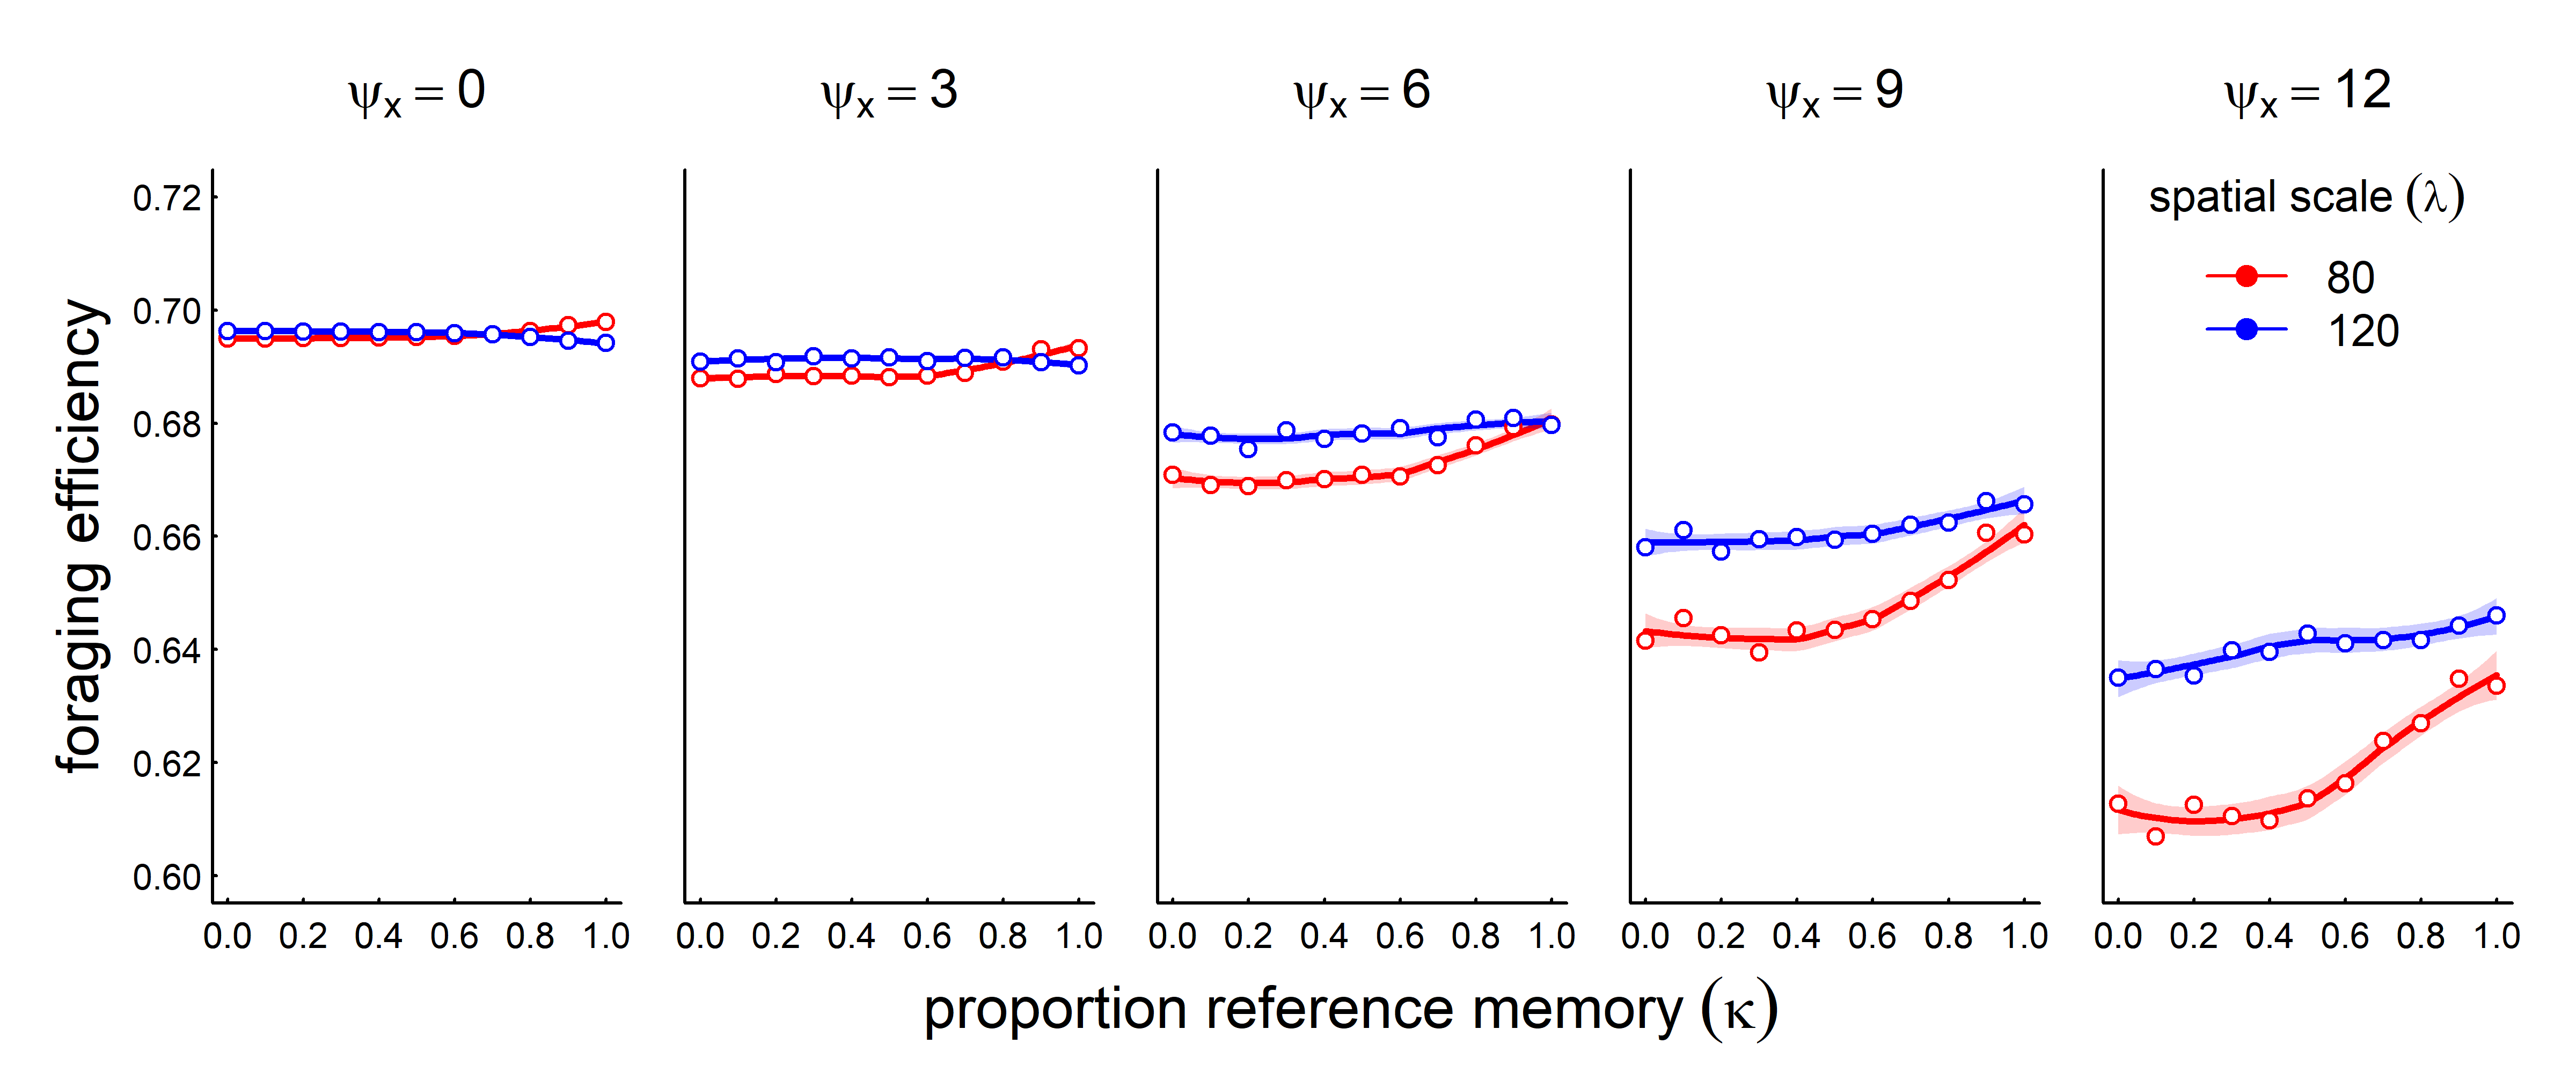
\includegraphics{figures/stochasticity.png}

\textbf{Figure 7} \emph{Foraging efficiency across various values of
reference memory \(\kappa\) (x-axis) for increasing amounts of
interannual stochasticity (\(\psi_x\), panels left to right), and two
values of spatial scale \(\lambda = 80\) and \(120\). For the stochastic
processes (\(\psi_x > 0\)), the process was run 30 times, and the mean
and standard error of the foraging efficiency over a 50 year
post-stabilization period is presented (points and bars). In these
scenarios, the resource following parameter \(\alpha = 100\), the social
attraction \(\beta = 400\) and diffusion \(\epsilon = 4\).} (NB: we are
running more replicated to get stronger results / narrower error bars
here)

\hypertarget{balancing-stochasticity-with-trends}{%
\subsection{Balancing stochasticity with
trends}\label{balancing-stochasticity-with-trends}}

We added trends to the stochastic process described above, adding 30
years of spatial outward trend in the resource. Our goal was to assess
the ability of the process to keep up with climate change as a function
of the reference memory parameter (Figure 8). Over-reliance on reference
memory (\(\kappa = 1\)) by definition does not allow the system to keep
up with climate change, leading to an adaptation index of 0. However, in
many cases a balancing of recent and reference memory (\(\kappa\) value
between 0.6 and 0.8) in many cases was slightly but significantly better
than relying entirely on recent memory. The smaller spatial scale (in
the selected parameter space) does a generally better job than the
larger spatial scale at lower stochasticity. At higher level of
stochasticity, however, the larger spatial scale outperforms the smaller
spatial scale, which completely loses track of the climate change.

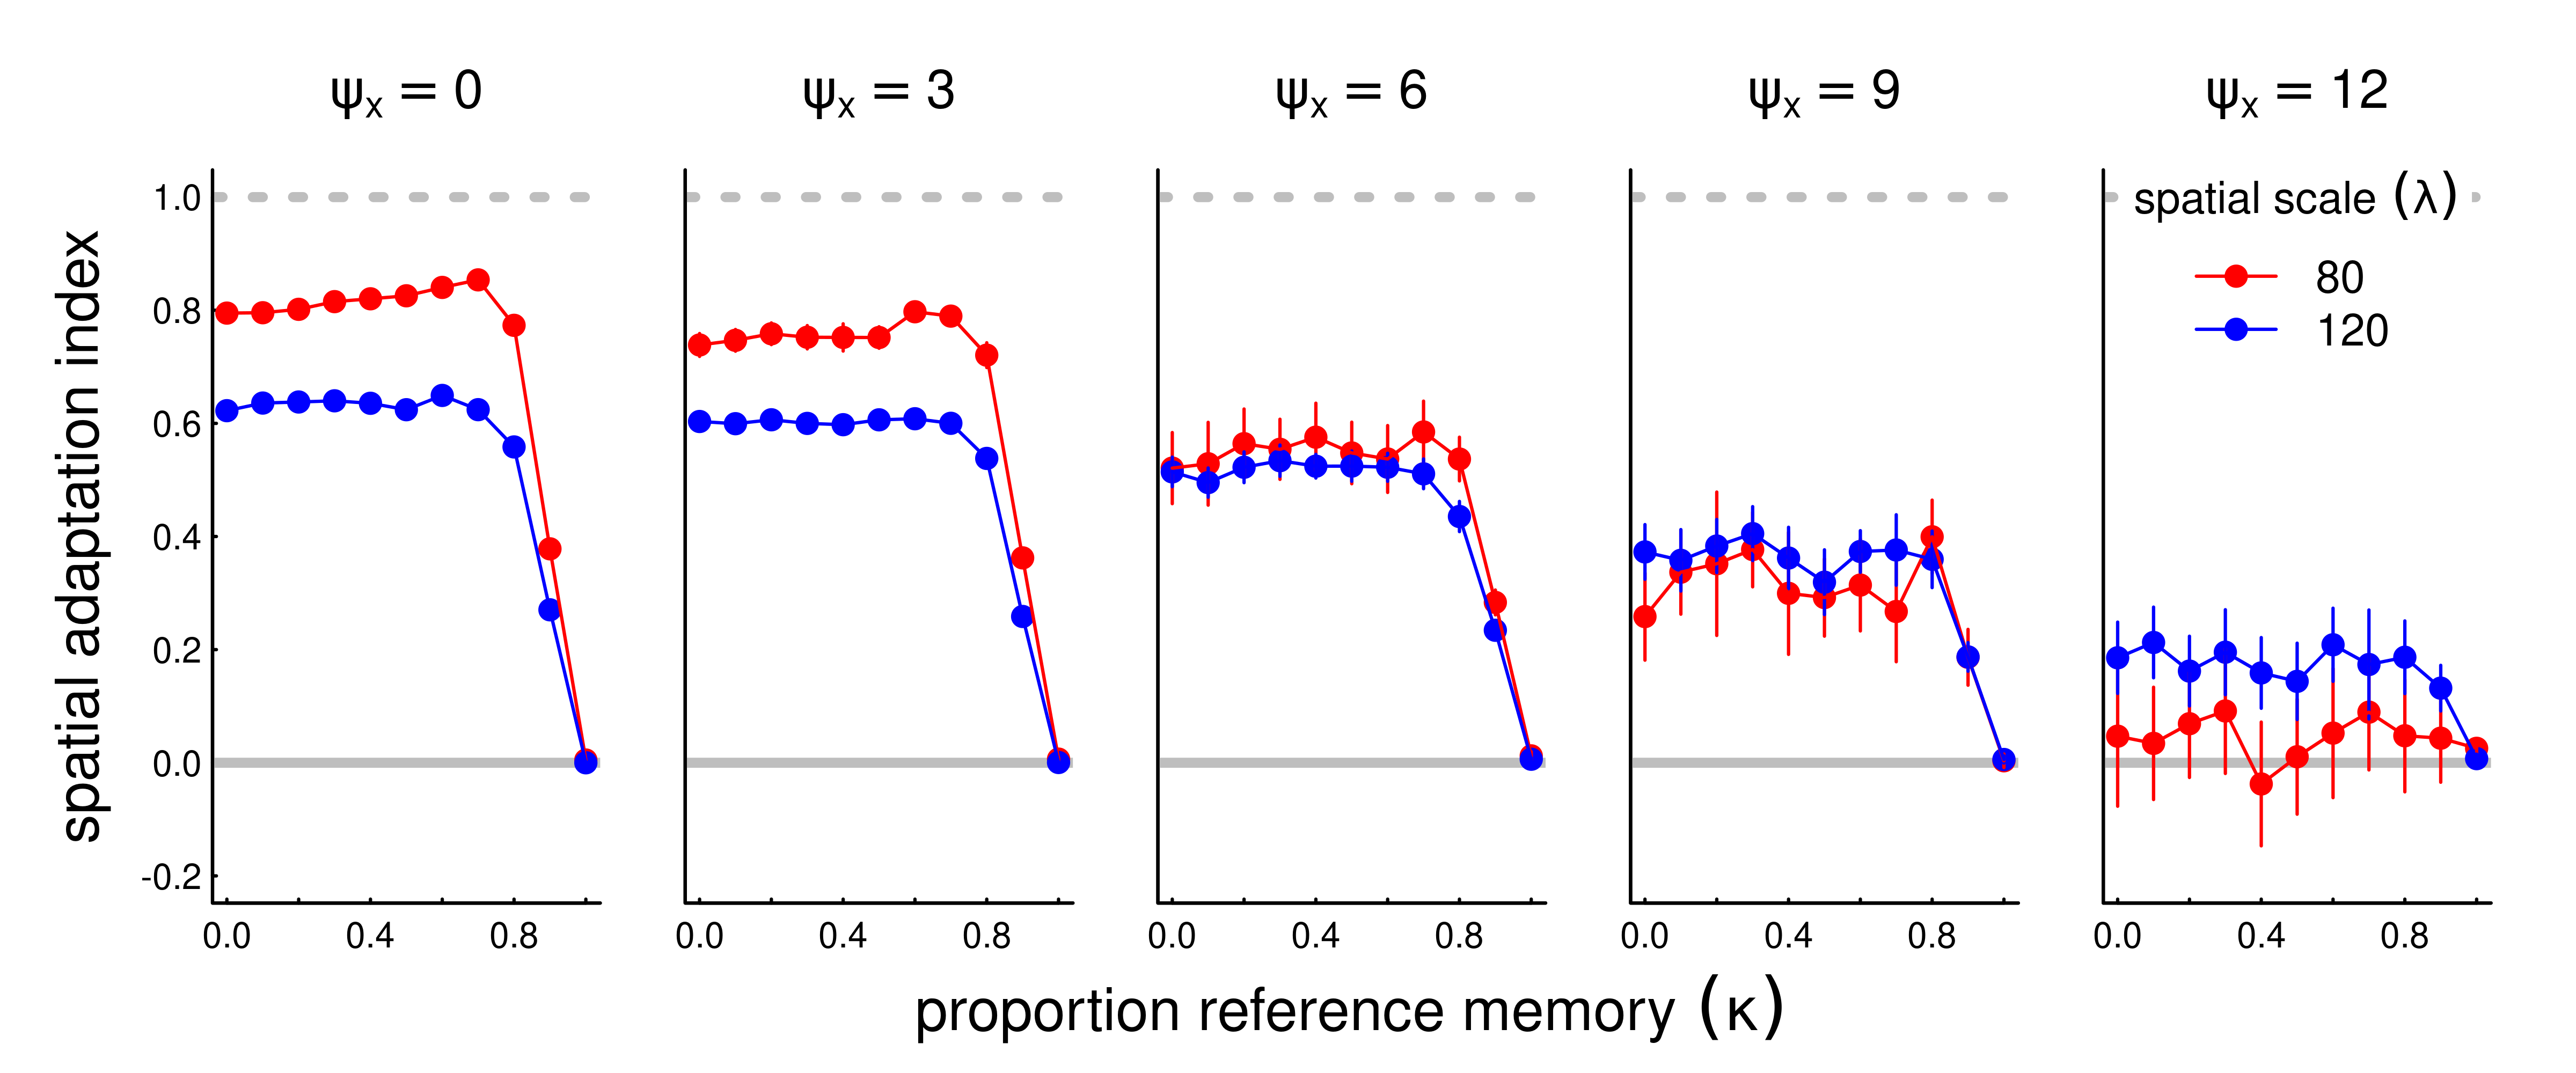
\includegraphics{figures/TrendStochasticity.png}

\textbf{Figure 8}. \emph{Role of reference memory in adapting to climate
change for increasingly stochastic resource dynamics. We ran the model
with a moderiate rate of climate change (mean shift: 0.5 / year) at five
increasing levels of stochasticity (inter-annual standard deviation of
resource peak 0, 3 ,6 and 12, left to right panels). For non-zero
stochasticity, we ran the process 30 times and present the mean and
standard error of the spatial adaptation index across various values of
the reference memory parameter \(\kappa\): where \(\kappa = 0\), the
system modifies its migration based entirely on recent experiences; at
\(\kappa = 1\), the memory never changes from the reference memory.
Other parameter values are resource following \(\alpha = 100\), social
attraction \(\beta = 400\), and social spatial scale \(\lambda = 80\).}

\hypertarget{discussion}{%
\section{Discussion}\label{discussion}}

Animals navigate complex, dynamic, patchy environments. When there is a
strongly localized and seasonal component to the resource dynamics,
typical strategies of spatial distribution by straightforward
resource-following taxis necessarily fails to maximally exploit the
dynamics. It is in these cases - quite common in the natural world -
that seasonal migration becomes a viable, even necessary, strategy.
However, when those resources start shifting in space and time - as is
occurring at an accelerated pace with recent global climate change - the
migration phenology itself must exhibit some plasticity. It is our
conjecture that this plasticity is greatly facilitated by a
memory-driven process, in which recent experiences inform strategic
behaviors in subsequent years. To our knowledge, this study is the first
attempt to focus in and propose a relatively simple, memory-driven
mechanism by which a population can respond to long-term changes in
resource dynamics.

We found that the straightforward inclusion of a migration-specific
memory in a social diffusion-advection framework was sufficient to
capture many fundamental phenomena related to migration. In essence, our
model allowed a population with a hybrid migratory and resource
following behavior to adjust the migratory behavior based on recent
experiences with the resource location. The model, while simple, was
able to emulate the successful navigation of an environment with
temporally and spatially isolated seasonal resource patches, the
spontaneous emergence of a migratory behavior, and intrinsic robustness
to changes in those environmental resources, whether steadily shifting
trends or inter-annual stochasticity. We postulated a process defined by
relatively few parameters, and explored the ability of the process to
navigate a fixed set of environments with the goal of understanding the
combinations of factors that lead to a resilient migration behavior. The
foraging efficiency was a convenient metric of the utility of the
migratory behavior, but was not a measure explicitly maximized by the
model.\\
A few rather general conclusions can be made from our model. One is that
migration in general can be acquired, as has been demonstrated for
translocated ungulates (Jesmer et al. 2018), even in environments where
resources are difficult to ``surf,'' but that this requires a very
strong attraction to resources, somewhat higher levels of exploratory
behavior, and many years. On the other hand, migrations can be
considered somewhat fragile, in the sense that under certain conditions,
e.g.~increasing stochasticity, rapidly shifting resources, or a shift in
some of the system parameters, migration can collapse down into a
localized non-migratory, residential behavior, at times with only a
marginal cost to the foraging efficiency index. This sensitivity may
explain why partially migratory populations composed of a mixture of
resident and migratory individuals are so common and, apparently,
evolutionary stable (Berthold 1999, Chapman et al. 2011).

We also found that the ability to maintain, learn and adapt migration
also depends strongly on properties of the resource dynamics. In
particular, the reinforcement of memory and foraging is strongest when
patches are concentrated in time, but relatively large in space.
Interestingly, in most stable patterns, the eventual targeted migration
arrival time coincided with the \emph{peak}, rather than the beginning,
of the resource dynamic. This indicates that the long-distance social
migration behavior may be particularly reinforced when the targeted
resource is very sudden (explosive), which is the case for the rapid
green-up that occurs in high latitudes as snow recedes in tandem with
extended day lengths, leading to a rapid and intense local green-up.

The sociality parameters - in particular, the spatial scale \(\lambda\)
- were somewhat unexpectedly, the most important for determining the
resiliency of the process for stabilizing a migratory behavior. In
particular, a very small spatial scale tended to have a much more
difficult time locking in to an adaptive migratory pattern, and only in
conditions where the social attraction was relatively weak. In order to
adapt to any shift in resources, \emph{some} individuals must experience
that resource, and the two sociality-related mechanisms to have that
scope is either a relatively large spatial scale or a relatively weak
social cohesion. On the other hand, overly large spatial scales
compromized the ability of the process to track climate change, due to a
diluting of the population's ability to concentrate over available
resource patches when made available.

All of the parameters in our model have well-defined biological
interpretations. The diffusion (\(\epsilon\)) captures short time-scaled
randomness of movement, capturing the exploratory and short-term
dispersive behavior. The foraging advection strength (\(\alpha\))
captures the attraction of the population to better quality resources at
a relatively large scale. These two parameters, the basic ingredients in
diffusion-advection models of animal movement, have direct parallels to
empirically estimated properties of animal behavior: diffusion is
closely related to families of random walk models (Gurarie and
Ovaskainen 2011) while the advective taxis is related to the step- and
resource selection functions that are routinely estimated from movement
datas (Potts and Schlägel 2020). The spatial scale of the social group
(\(\lambda\)) captures the spatial extent of the population, i.e.~a
population-level range. The sociality parameter (\(\beta\)) quantifies
the strength an individual's desire to approach the center of the social
group. This is not a parameter that is typically measured, though it
would - in principle - be possible to estimate in a manner analogous to
step-selection function using only other conspecifics as opposed to
environmental variables as a covariate. Because both resources and
populations were normalized to 1, the ratio between \(\beta\) and
\(\alpha\) can be interpreted as the relative importance of foraging to
social cohesion. It does appears a certain balance of both is needed to
successfully maintain, acquire, or adapt a migratory phenology. Finally,
the migration timing and location parameter can be similarly
straightforwardly estimated from movement data (Cagnacci et al. 2015,
Gurarie et al. 2019). Thus, for example, Gurarie et al. (2019)
explicitly esimated the ranging area, timing, and seasonal range
locations for migratory caribou (\emph{Rangifer tarandus}), identifying
the kind of inter-annual variation that is reflected in the stochastic
scenarios explored here as well as some trends in the timing of
migration. Finally, we note that our underlying assumption of the
migration ``urge'' is consistent with the strong endogenous programs to
migrate taht is well-documented, in particular, in birds that exhibit a
seasonal restlessness known as \emph{Zugunruhe} (Berthold 1999, Helm
2006).

Collective knowledge has been shown to be important, if not essential,
to the evolution and process of migration (Guttal and Couzin 2010, Shaw
and Couzin 2013, Berdahl et al. 2018). In our model, we assume that the
migration process itself is driven by a collective trigger for the
timing and locations of seasonal ranges and migration behavior.
Synchrony of migration timing and high site fidelity are well documented
for migratory species (Gurarie et al. 2019, Joly et al. 2021). We note,
however, that diffusion-advection models can also be interpreted as a
probabilistic description of a single individual's movement. In this
case, \(\lambda\) would correspond to an individual home-range and
\(\beta\) would be an individual's tendency to be drawn to the center of
that home range, akin to an individual migratory Ornstein-Uhlenbeck
process (Gurarie et al. 2017).

The reference memory parameter \(\kappa\) is, of course, impossible to
observe directly. Our model does, however, allow us to explore in an
heuristic way the conditions under which a strong cultural tendency to
migrate with certain fixed patterns can help a population hedge against
stochasticity. In general, our model allows us to consider broadly the
risks.

Importantly, our model did not include any selection, inheritance or
birth or death processes, i.e.~there was no evolutionary maximization of
a fitness, as in many models that explicitly explore the evolution of
migration (e.g. Guttal and Couzin 2010, Anderson et al. 2013, Shaw and
Couzin 2013). Nonetheless, it is instructive to compare the fundamental
assumptions behind such evolutionary individual-based models and a
social memory-based model like ours. For example, Anderson et al. (2013)
similarly explored the resilience of a population under selective
pressure under persistent trends and increased stochasticity of a
drifting optimal resource window, showing that a certain amount of
heritable phenotypic plasticity is necessary to adapt successfully to
climate change even at the cost of efficiency. Our model underscores the
fact that some level of resilience and adapatability can be attained
with a purely cognitive process that balances sociality, long, and short
term collective memory. Importantly, this knowledge must be transmitted
through social and cultural, rather than genetic, pathways. The high
level of sociality among migratory animals, as well as multi-annual
parent offspring bonds, are an evident pathway for that kind of
transmission. As with those evolutionary models, however, it is clear
that when changes are too rapid, no amount of cognition can help
entirely mitigate against adverse outcomes. Furthermore, if behaviors
are not sufficiently plastic (i.e.~if \(\kappa\) is too close to 1),
then adaptation is that much more difficult.

Rapid environmental change, both global warming and increased
anthropogenic development, is causing severe and dramatic impacts to the
widespread and generally successful strategy of seasonal migration for
many taxa, and the fate of many animal migrations is a topic of
increasing concern (Wilcove and Wikelski 2008, Kauffman et al. 2021).
The ability of animals to respond to these changes is deeply dependent
on their behavioral plasticity and cognitive abilities. The importance
of those abilities are in direct proportion to the difficulty in
studying them directly. By quantitatively exploring the properties of a
heuristic model that distill many of the main properties of wild
populations in dynamic and seasonal environments, we hope to have
identified some broad patterns that might guide further empirical
exploration of the cognitive underpinnings of adapatability and
resilience.

\hypertarget{acknowledgments}{%
\section{Acknowledgments}\label{acknowledgments}}

NSF grant. Quentin at SESYNC.

\hypertarget{references}{%
\section*{References}\label{references}}
\addcontentsline{toc}{section}{References}

\hypertarget{refs}{}
\begin{CSLReferences}{1}{0}
\leavevmode\hypertarget{ref-Abrahms2019}{}%
Abrahms, B., E. L. Hazen, E. O. Aikens, M. S. Savoca, J. A. Goldbogen,
S. J. Bograd, M. G. Jacox, L. M. Irvine, D. M. Palacios, and B. R. Mate.
2019. Memory and resource tracking drive blue whale migrations.
Proceedings of the National Academy of Sciences 116:5582--5587.

\leavevmode\hypertarget{ref-Anderson2013}{}%
Anderson, J. J., E. Gurarie, C. Bracis, B. J. Burke, and K. L. Laidre.
2013. Modeling climate change impacts on phenology and population
dynamics of migratory marine species. Ecological Modelling 264:83--97.

\leavevmode\hypertarget{ref-Avgar2014}{}%
Avgar, T., G. Street, and J. M. Fryxell. 2014. On the adaptive benefits
of mammal migration. Canadian Journal of Zoology 92:481--490.

\leavevmode\hypertarget{ref-Berdahl2018}{}%
Berdahl, A. M., A. B. Kao, A. Flack, P. A. Westley, E. A. Codling, I. D.
Couzin, A. I. Dell, and D. Biro. 2018. Collective animal navigation and
migratory culture: From theoretical models to empirical evidence.
Philosophical Transactions of the Royal Society B: Biological Sciences
373:20170009.

\leavevmode\hypertarget{ref-Berthold1999}{}%
Berthold, P. 1999. A comprehensive theory for the evolution, control and
adaptability of avian migration. Ostrich 70:1--11.

\leavevmode\hypertarget{ref-Bhattacharyya1943}{}%
Bhattacharyya, A. 1943. On a measure of divergence between two
statistical populations defined by their probability distributions.
Bull. Calcutta Math. Soc. 35:99--109.

\leavevmode\hypertarget{ref-Bischof2012}{}%
Bischof, R., L. E. Loe, E. L. Meisingset, B. Zimmermann, B. Van Moorter,
and A. Mysterud. 2012. A migratory northern ungulate in the pursuit of
spring: Jumping or surfing the green wave? The American Naturalist
180:407--424.

\leavevmode\hypertarget{ref-Bracis2017}{}%
Bracis, C., and T. Mueller. 2017. Memory, not just perception, plays an
important role in terrestrial mammalian migration. Proceedings of the
Royal Society B: Biological Sciences 284:20170449.

\leavevmode\hypertarget{ref-Breiman2001}{}%
Breiman, L. 2001. Random forests. Machine learning 45:5--32.

\leavevmode\hypertarget{ref-Cagnacci2015}{}%
Cagnacci, F., S. Focardi, A. Ghisla, B. van Moorter, E. H. Merrill, E.
Gurarie, M. Heurich, A. Mysterud, J. Linnell, M. Panzacchi, R. May, T.
Nygård, C. Rolandsen, and M. Hebblewhite. 2015. How many routes lead to
migration? Comparison of methods to assess and characterize migratory
movements. Journal of Animal Ecology 85:54--68.

\leavevmode\hypertarget{ref-Chapman2011}{}%
Chapman, B. B., C. Brönmark, J.-Å. Nilsson, and L.-A. Hansson. 2011. The
ecology and evolution of partial migration. Oikos 120:1764--1775.

\leavevmode\hypertarget{ref-Dingle2014}{}%
Dingle, H. 2014. Migration: The biology of life on the move. Oxford
University Press, USA.

\leavevmode\hypertarget{ref-minpack.lm}{}%
Elzhov, T. V., K. M. Mullen, A.-N. Spiess, and B. Bolker. 2016.
Minpack.lm: R interface to the levenberg-marquardt nonlinear
least-squares algorithm found in MINPACK, plus support for bounds.

\leavevmode\hypertarget{ref-Fagan2017}{}%
Fagan, W., E Gurarie, S. Bewick, A. Howard, R. Cantrell, and C. Cosner.
2017. Perceptual ranges, information gathering, and foraging success in
dynamic landscapes. The American Naturalist 189:474--489.

\leavevmode\hypertarget{ref-Fagan2019}{}%
Fagan, W., T. Hoffman, D. Dahiya, E Gurarie, R. Cantrell, and C. Cosner.
2019. Improved foraging by switching between diffusion and advection:
Benefits from movement that depends on spatial context. Theoretical
Ecology 13:127--136.

\leavevmode\hypertarget{ref-Fryxell1988}{}%
Fryxell, J. M., J. Greever, and A. Sinclair. 1988. Why are migratory
ungulates so abundant? The American Naturalist 131:781--798.

\leavevmode\hypertarget{ref-Gurarie2009}{}%
Gurarie, E., J. J. Anderson, and R. W. Zabel. 2009. Continuous models of
population-level heterogeneity inform analysis of animal dispersal and
migration. Ecology 90:2233--2242.

\leavevmode\hypertarget{ref-Gurarie2017}{}%
Gurarie, E., F. Cagnacci, W. Peters, C. H. Fleming, J. M. Calabrese, T.
Mueller, and W. F. Fagan. 2017. A framework for modelling range shifts
and migrations: Asking when, whither, whether and will it return.
Journal of Animal Ecology 86:943--959.

\leavevmode\hypertarget{ref-Gurarie2017}{}%
Gurarie, E., F. Cagnacci, W. Peters, C. H. Fleming, J. M. Calabrese, T.
Mueller, and W. F. Fagan. 2017. A framework for modelling range shifts
and migrations: Asking when, whither, whether and will it return.
Journal of Animal Ecology 86:943--959.

\leavevmode\hypertarget{ref-Gurarie2019}{}%
Gurarie, E., M. Hebblewhite, K. Joly, A. P. Kelly, J. Adamczewski, S. C.
Davidson, T. Davison, A. Gunn, M. J. Suitor, W. F. Fagan, and others.
2019. Tactical departures and strategic arrivals: Divergent effects of
climate and weather on caribou spring migrations. Ecosphere 10:e02971.

\leavevmode\hypertarget{ref-Gurarie2011}{}%
Gurarie, E., and O. Ovaskainen. 2011. Characteristic spatial and
temporal scales unify models of animal movement. The American Naturalist
178:113--123.

\leavevmode\hypertarget{ref-Guttal2010}{}%
Guttal, V., and I. D. Couzin. 2010. Social interactions, information
use, and the evolution of collective migration. Proceedings of the
National Academy of Sciences 107:16172--16177.

\leavevmode\hypertarget{ref-Helm2006}{}%
Helm, B. 2006. Zugunruhe of migratory and non-migratory birds in a
circannual context. Journal of Avian Biology 37:533--540.

\leavevmode\hypertarget{ref-Jesmer2018}{}%
Jesmer, B. R., J. A. Merkle, J. R. Goheen, E. O. Aikens, J. L. Beck, A.
B. Courtemanch, M. A. Hurley, D. E. McWhirter, H. M. Miyasaki, K. L.
Monteith, and others. 2018. {Is ungulate migration culturally
transmitted? Evidence of social learning from translocated animals}.
Science 361:1023--1025.

\leavevmode\hypertarget{ref-Joly2021}{}%
Joly, K., E. Gurarie, D. A. Hansen, and M. D. Cameron. 2021. Seasonal
patterns of spatial fidelity and temporal consistency in the
distribution and movements of a migratory ungulate. Ecology and
Evolution 11:8183--8200.

\leavevmode\hypertarget{ref-Kauffman2021}{}%
Kauffman, M. J., F. Cagnacci, S. Chamaillé-Jammes, M. Hebblewhite, J. G.
C. Hopcraft, J. A. Merkle, T. Mueller, A. Mysterud, W. Peters, C.
Roettger, A. Steingisser, J. E. Meacham, K. Abera, J. Adamczewski, E. O.
Aikens, H. Bartlam-Brooks, E. Bennitt, J. Berger, C. Boyd, S. D. Côté,
L. Debeffe, A. S. Dekrout, N. Dejid, E. Donadio, L. Dziba, W. F. Fagan,
C. Fischer, S. Focardi, J. M. Fryxell, R. W. S. Fynn, C. Geremia, B. A.
González, A. Gunn, E. Gurarie, M. Heurich, J. Hilty, M. Hurley, A.
Johnson, K. Joly, P. Kaczensky, C. J. Kendall, P. Kochkarev, L.
Kolpaschikov, R. Kowalczyk, F. van Langevelde, B. V. Li, A. L. Lobora,
A. Loison, T. H. Madiri, D. Mallon, P. Marchand, R. A. Medellin, E.
Meisingset, E. Merrill, A. D. Middleton, K. L. Monteith, M. Morjan, T.
A. Morrison, S. Mumme, R. Naidoo, A. Novaro, J. O. Ogutu, K. A. Olson,
A. Oteng-Yeboah, R. J. A. Ovejero, N. Owen-Smith, A. Paasivaara, C.
Packer, D. Panchenko, L. Pedrotti, A. J. Plumptre, C. M. Rolandsen, S.
Said, A. Salemgareyev, A. Savchenko, P. Savchenko, H. Sawyer, M.
Selebatso, M. Skroch, E. Solberg, J. A. Stabach, O. Strand, M. J.
Suitor, Y. Tachiki, A. Trainor, A. Tshipa, M. Z. Virani, C. Vynne, S.
Ward, G. Wittemyer, W. Xu, and S. Zuther. 2021. Mapping out a future for
ungulate migrations. Science 372:566--569.

\leavevmode\hypertarget{ref-Kot1996}{}%
Kot, M., M. A. Lewis, and P. van der Driessche. 1996. Dispersal data and
the spread of invading organisms. Ecology 77:2027--2042.

\leavevmode\hypertarget{ref-Kolzsch2015}{}%
Kölzsch, A., S. Bauer, R. De Boer, L. Griffin, D. Cabot, K.-M. Exo, H.
P. Van der Jeugd, and B. A. Nolet. 2015. {Forecasting spring from afar?
Timing of migration and predictability of phenology along different
migration routes of an avian herbivore}. Journal of Animal Ecology
84:272--283.

\leavevmode\hypertarget{ref-Lin2021}{}%
Lin, H.-Y., W. F. Fagan, and P.-E. Jabin. 2021. Memory-driven movement
model for periodic migrations. Journal of Theoretical Biology
508:110486.

\leavevmode\hypertarget{ref-Mogilner1999}{}%
Mogilner, A., and L. Edelstein-Keshet. 1999. A non-local model for a
swarm. Journal of Mathematical Biology 38:534--570.

\leavevmode\hypertarget{ref-Okubo2001}{}%
Okubo, A., and S. Levin. 2001. {Diffusion and Ecological Problems:
Modern Perspectives}. Springer Verlag, New York.

\leavevmode\hypertarget{ref-Potts2020}{}%
Potts, J. R., and U. E. Schlägel. 2020. Parametrizing diffusion-taxis
equations from animal movement trajectories using step selection
analysis. Methods in Ecology and Evolution 11:1092--1105.

\leavevmode\hypertarget{ref-Robinson2009}{}%
Robinson, R., H. Crick, J. Learmonth, I. Maclean, C. Thomas, F.
Bairlein, M. Forchhammer, C. Francis, J. Gill, B. Godley, J. Harwood, G.
Hays, B. Huntley, A. Hutson, G. Pierce, M. Rehfisch, D. Sims, B. Santos,
T. Sparks, D. Stroud, and M. Visser. 2009. Travelling through a warming
world: Climate change and migratory species. Endangered Species Research
7:87--99.

\leavevmode\hypertarget{ref-Shaw2016}{}%
Shaw, A. K. 2016. Drivers of animal migration and implications in
changing environments. Evolutionary Ecology 30:991--1007.

\leavevmode\hypertarget{ref-Shaw2013}{}%
Shaw, A. K., and I. D. Couzin. 2013. Migration or residency? The
evolution of movement behavior and information usage in seasonal
environments. The American Naturalist 181:114--124.

\leavevmode\hypertarget{ref-Skalski2003}{}%
Skalski, G. T., and J. F. Gilliam. 2003. A diffusion-based theory of
organism dispersal in heterogeneous populations. The American Naturalist
161:441--458.

\leavevmode\hypertarget{ref-Skellam1951}{}%
Skellam, J. G. 1951. Random dispersal in theoretical populations.
Biometrika 38:196--218.

\leavevmode\hypertarget{ref-Soetaert2012}{}%
Soetaert, K., and F. Meysman. 2012. {Reactive transport in aquatic
ecosystems: Rapid model prototyping in the open source software R}.
Environmental Modelling \& Software 32:49--60.

\leavevmode\hypertarget{ref-Soetaert2010}{}%
Soetaert, K., T. Petzoldt, and R. W. Setzer. 2010. Solving differential
equations in {R}: Package de{S}olve. Journal of Statistical Software
33:1--25.

\leavevmode\hypertarget{ref-Turchin1998}{}%
Turchin, P. 1998. Quantitative analysis of movement: Measuring and
modeling population redistribution in animals and plants. Sinauer
Associates.

\leavevmode\hypertarget{ref-Wilcove2008}{}%
Wilcove, D. S., and M. Wikelski. 2008. Going, going, gone: Is animal
migration disappearing. {PLoS} Biology 6:e188.

\leavevmode\hypertarget{ref-Wilcove2008}{}%
Wilcove, D. S., and M. Wikelski. 2008. Going, going, gone: Is animal
migration disappearing. {PLoS} Biology 6:e188.

\end{CSLReferences}

\end{document}
